\documentclass[10pt]{article}
\usepackage[letterpaper]{geometry}
\geometry{verbose,tmargin=1in,bmargin=1in,lmargin=1in,rmargin=1in}
\usepackage{setspace}
\usepackage{ragged2e}
\usepackage{algorithm2e,etoolbox}
\AtBeginEnvironment{algorithm}{\let\textnormal\ttfamily\DontPrintSemicolon}
\usepackage{color, colortbl}
\usepackage{titlesec}
\usepackage{graphicx}
\usepackage{float}
\usepackage{mathtools}
\usepackage{amsmath}
\usepackage[font=small,labelfont=bf,labelsep=period]{caption}
\usepackage[english]{babel}
\usepackage{indentfirst}
\usepackage{array}
\usepackage{makecell}
\usepackage[usenames,dvipsnames]{xcolor}
\usepackage{multirow}
\usepackage{tabularx}
\usepackage{arydshln}
\usepackage{caption}
\usepackage{subcaption}
\usepackage{xfrac}
\usepackage{etoolbox}
\usepackage{cite}
\usepackage{url}
\usepackage{dcolumn}
\usepackage{hyperref}
\usepackage{courier}
\usepackage{url}
\usepackage{esvect}
\usepackage{commath}
\usepackage{verbatim} % for block comments
\usepackage{enumitem}
\usepackage{hyperref} % for clickable table of contents
\usepackage{braket}
\usepackage{titlesec}
\usepackage{booktabs}
\usepackage{gensymb}
\usepackage{longtable}
\usepackage{glossaries}
\usepackage{tcolorbox} % for colored boxes
\tcbuselibrary{breakable} % to allow colored boxed to extend over multiple pages
\usepackage[mathscr]{euscript} % for script letters
\usepackage{wasysym}  % for checkboxes
\usepackage{bm} % for bolding math symbols
\usepackage{listings} % for including code in boxes
\setcounter{MaxMatrixCols}{20} % sets max matrix length as 20 columns

\lstdefinestyle{mystyle}{ 
    commentstyle=\color{gray},
    keywordstyle=\color{magenta},
    stringstyle=\color{orange},
    basicstyle=\footnotesize,
    language=C++,
    breakatwhitespace=false,         
    breaklines=true,                 
    captionpos=b,                    
    keepspaces=true,                                                  
    showspaces=false,                
    showstringspaces=false,
    showtabs=false,          
    basicstyle=\small\ttfamily,        
    tabsize=2
}

\lstset{style=mystyle}

% change spacing around sections
\titlespacing*{\section}
{0pt}{8ex}{1ex}
\titlespacing*{\subsection}
{0pt}{5ex}{1ex}

% new commands for shorter writing of equations
\newcommand{\beq}{\begin{equation}}
\newcommand{\eeq}{\end{equation}}
\newcommand{\beqa}{\begin{equation}\begin{aligned}}
\newcommand{\eeqa}{\end{aligned}\end{equation}}

% Acronyms used
\setacronymstyle{long-short}
\newacronym{anl}{ANL}{Argonne National Laboratory}
\newacronym{cfd}{CFD}{Computational Fluid Dynamics}
\newacronym{fe}{FE}{Finite Element}
\newacronym{fem}{FEM}{Finite Element Method}
\newacronym{inl}{INL}{Idaho National Laboratory}
\newacronym{io}{I/O}{Input/Output}
\newacronym{moon}{MOON}{MOOSE and Nek}
\newacronym{moose}{MOOSE}{the Multiphysics Object-Oriented Simulation Environment}

\titleclass{\subsubsubsection}{straight}[\subsection]

% define new command for triple sub sections
\newcounter{subsubsubsection}[subsubsection]
\renewcommand\thesubsubsubsection{\thesubsubsection.\arabic{subsubsubsection}}
\renewcommand\theparagraph{\thesubsubsubsection.\arabic{paragraph}} % optional; useful if paragraphs are to be numbered

\titleformat{\subsubsubsection}
  {\normalfont\normalsize\bfseries}{\thesubsubsubsection}{1em}{}
\titlespacing*{\subsubsubsection}
{0pt}{3.25ex plus 1ex minus .2ex}{1.5ex plus .2ex}

\makeatletter
\renewcommand\paragraph{\@startsection{paragraph}{5}{\z@}%
  {3.25ex \@plus1ex \@minus.2ex}%
  {-1em}%
  {\normalfont\normalsize\bfseries}}
\renewcommand\subparagraph{\@startsection{subparagraph}{6}{\parindent}%
  {3.25ex \@plus1ex \@minus .2ex}%
  {-1em}%
  {\normalfont\normalsize\bfseries}}
\def\toclevel@subsubsubsection{4}
\def\toclevel@paragraph{5}
\def\toclevel@paragraph{6}
\def\l@subsubsubsection{\@dottedtocline{4}{7em}{4em}}
\def\l@paragraph{\@dottedtocline{5}{10em}{5em}}
\def\l@subparagraph{\@dottedtocline{6}{14em}{6em}}
\makeatother

\newcommand{\volume}{\mathop{\ooalign{\hfil$V$\hfil\cr\kern0.08em--\hfil\cr}}\nolimits}

\numberwithin{equation}{section} % for equation numbering

\setcounter{secnumdepth}{4}
\setcounter{tocdepth}{4}
\makeglossaries
\begin{document}

\title{OpenMC, BISON, and Nek Coupling}
\author{Argonne National Laboratory}
\maketitle

\tableofcontents
%\printglossary[type=\acronymtype,title=Abbreviations]

\clearpage

\section{Introduction}

This document is intended to describe the coupling methodology between Nek, a \gls{cfd} code developed by \gls{anl}, OpenMC, a Monte Carlo code developed by \gls{anl}, and BISON, a nuclear fuel performance code developed by \gls{inl}. Previous work by Matthew Ellis and others at MIT resulted in the coupling of OpenMC to MOOSE, and work by a joint effort of \gls{anl} and \gls{inl} resulted in the coupling of Nek to MOOSE. So, the coupling of all three codes together will attempt to utilize as much as possible regarding this previous work. The purpose of this report is to document the coupling process, justify decisions made, and illustrate how to use these codes in a coupled manner. The input files for a working three-way example are discussed in Section \ref{sec:BuildConfig}.

This report is organized beginning with a description of the overall coupling methodology, followed by a discussion of the nuts-and-bolts requirements for coupling two codes in terms of the data transfer between the codes and executing non-MOOSE codes from within the MOOSE framework. Finally, the end of this document discusses the mechanics of coupling the three codes together in terms of the build configuration. This document serves as my working notes, so any lingering ``dangers'' that are not fully resolved are indicated in pink font.

\clearpage
\section{Overall Coupling Methodology}
This section discusses the overall coupling methodology that was pursued between OpenMC-BISON, BISON-Nek, and finally OpenMC-BISON-Nek. The immediate jump to the coupling of all three codes was not performed because taking smaller steps often helps reveal difficulties that would otherwise be compounded and confusing when performing the full three-way coupling. When coupling two distinct projects, there are generally three ways to perform the coupling:

\begin{enumerate}
\item Make virtually no changes to the source code either project, but write an external script that will:
	\begin{enumerate}
	\item Run the first code.
	\item Read the text output file of the first code and modify the text input file for the second code.
	\item Run the second code.
	\item Read the text output file of the second code and modify the text input file for the first code. 
	\item Repeat (a)-(d) until convergence, then move to the next time step.
	\end{enumerate}
	This approach is necessary for projects that restrict access to source code, since a more internal coupling requires modifications to the source code of one or more of the projects. The only interaction with the software with this method is through text files.
\item Write a custom driver that will call routines from each code. This may be fast to develop, but limits the reusability of the driver itself or changes made to the two codes to meld to the driver structure. For example, pseudo-code for a driver written to couple OpenMC and Nek may have the following overall structure:

	\begin{algorithm}[H]
	{\tt initialize OpenMC}\;
	{\tt initialize Nek}\;
	\;
	\While{t $<$ end time}{
	  \While{not converged}{
	    run OpenMC\;
	    transfer data to Nek\;
	    run Nek\;
	    transfer data to OpenMC\;
	    evaluate convergence\;
	  }
	  advance time state\;
	}
	\end{algorithm}
	
\item Use an existing driver with a sufficiently general structure that the codes you want to couple can be structurally changed to be composed of routines that can be called from within the existing driver (no editing of text files). This approach, by virtue of using an existing driver, allows you to immediately take advantage of the ability to couple to any other codes that have been cast in terms of that driver's methods. However, this approach requires a good understanding of the existing driver, which can be much more time consuming than developing a custom driver from scratch. In addition, using an existing coupling framework can potentially restrict control over parallelism and performance, since the driver structure may not be ideal for every application.
\end{enumerate}

Adapting OpenMC and Nek to an existing driver framework was selected for this work for the reasons given above. Work at ANL has simultaneously worked towards developing a custom driver to run OpenMC and Nek, but this will not be discussed here. The MOOSE framework was selected as the driver for the following reasons:

\begin{enumerate}
\item Many applications have been developed with the MOOSE framework, such as nuclear fuels simulations (BISON), porous media thermal-hydraulics (PRONGHORN), and many other physics. Using the MOOSE coupling framework allows OpenMC and Nek to essentially become "MOOSE" Animals in that they can not only be coupled to each other, as the scope of this project seeks, but to these other codes with relatively minor effort.
\item Significant work has already been performed with coupling OpenMC to MOOSE and Nek to MOOSE, so the coupling of OpenMC with Nek in principle can directly take advantage of this existing work.
\item The MOOSE framework is easy-to-use and has significant coupling capabilities already developed, as well as an accessible development team for assistance.
\end{enumerate}

If the parallel performance is not acceptable, then the work developed in constructing OpenMC and Nek as MOOSE applications can still be reused for a custom driver due to MOOSE's modular structure. The MOOSE coupling framework performs coupling in a tree-like structure. A Master App controls the entire coupled solve, and is the App that performs actions such as initializing MPI and transferring data amongst all of the Apps. For the Master App, there may be any number of sub-applications. The terminology "Sub-app" and "MultiApp" are essentially the same, where the use of sub app is used primarily to denote that a MultiApp is "down-the-tree" from another MultiApp. 

\begin{figure}[H]
\centering
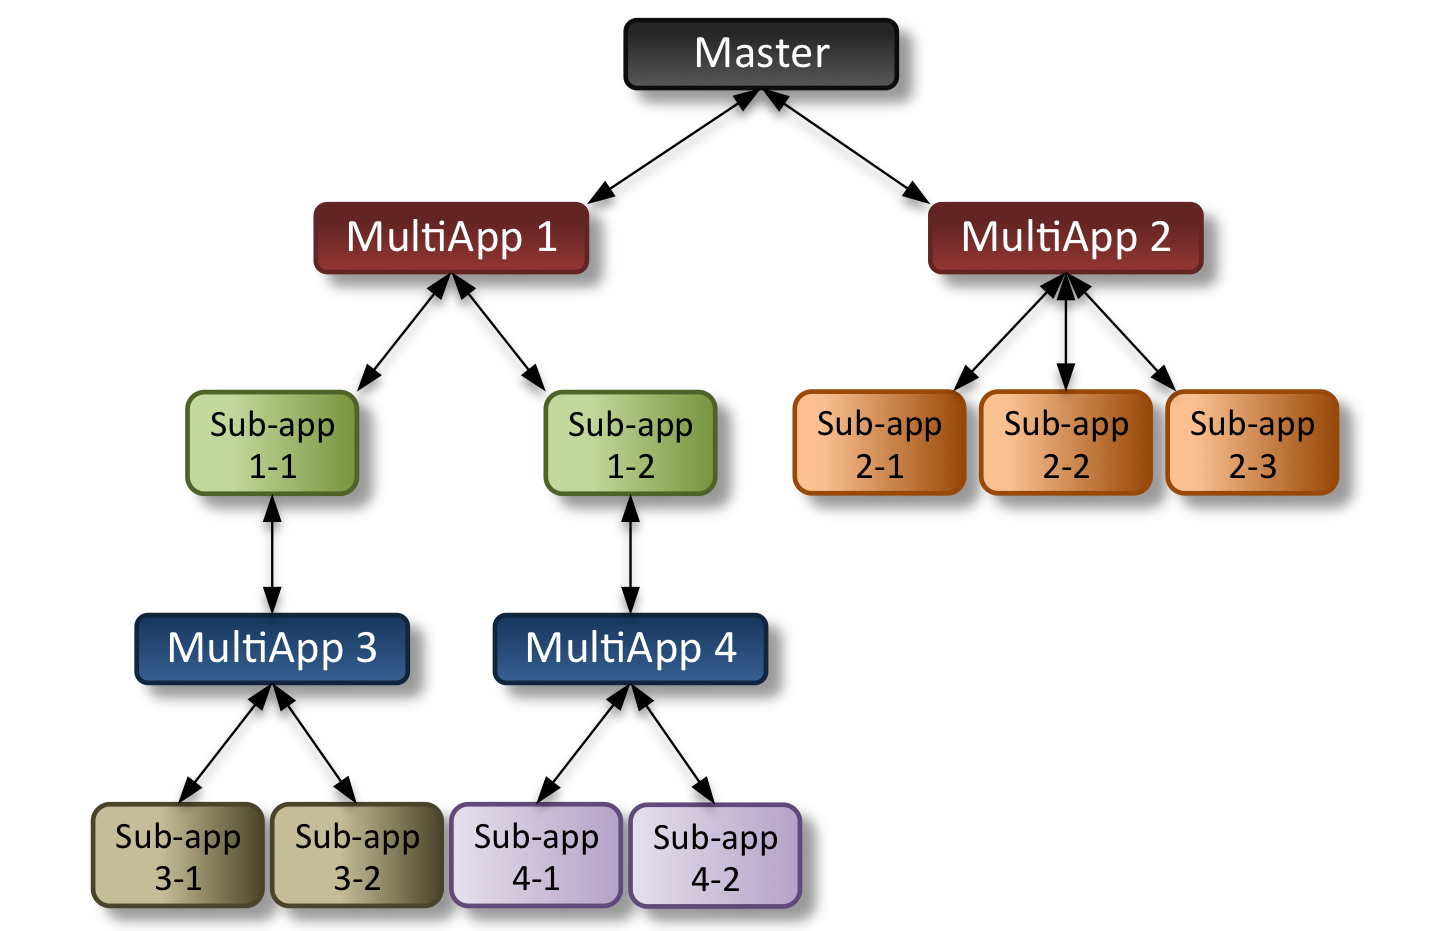
\includegraphics[width=10cm]{figures/multiapp_hierarchy.png}
\caption{MasterApp and MultiApp structure for a MOOSE simulation.}
\end{figure}

When using the MOOSE coupling framework, decisions must be made regarding the Master App-Multi App structure, such as which App acts as the Master App, and which as the Multi Apps. When only two codes are coupled, this choice is arbitrary, but when three or more codes are coupled this choice becomes important in determining the coupling structure, as will be discussed later. The remainder of this section discusses the high-level coupling strategy for OpenMC-MOOSE, Nek-MOOSE, and finally OpenMC-Nek-BISON. 

\subsection{OpenMC and BISON Coupling}
This section discusses the OpenMC-BISON coupling illustrated through an example that can be found in {\tt okapimcs/tests/FETs/bison-openmc}. This coupling is performed here using MOOSE as the Master App and Okapi and BISON as peer MultiApps, but because BISON is already a MOOSE Animal, this coupling can also be performed using BISON as the Master App and Okapi as the MultiApp (though this would only work for one fuel pin, since there cannot be multiple instances of the Master App). As an aside, to be fully explicit, you cannot have ``MOOSE'' as the Master App, since it just the framework. A Moose App must be the Master App, so when MOOSE is referred to as the Master App, this means that one of the Moose Apps used in the simulation is also used as the Master App, but it does not perform any physics solves, but just exists to pass data. For this implementation, Okapi is both the Master App and a Multi App.

Finally, because the later three-way coupling uses Okapi as the Master App, this coupling can {\it also} be performed with BISON as the MultiApp and Okapi the Master App. The remainder of the discussion in this section assumes a MOOSE Master App, and BISON and Okapi peer MultiApps, and the details would only be slightly modified to discuss these other configurations. OpenMC is wrapped as a MOOSE App so that it can be called as a MultiApp to the BISON Master App. BISON is already a MOOSE animal, and hence does not require any wrapping.

In a coupled solve, the following steps occur. We arbitrarily choose OpenMC to execute before BISON, so we choose to execute OpenMC on {\tt timestep\_begin}, and BISON on {\tt timestep\_end}. 

\begin{enumerate}
\item Initialize the MasterApp. The MasterApp does not perform any solves, but only exists to transfer data between its MultiApps.
\item Initialize OpenMC. This calls the {\tt OpenMCExecutioner::init()} method, which performs the regular initialization steps for any MOOSE App, followed by calling the {\tt openmc\_init} subroutine found in the OpenMC source. This subroutine performs basic tasks such as reading in the XML files that control OpenMC parameters (none are set in the MOOSE input files), allocating memory for data structures, etc.
\item Initialize BISON. Because BISON is a Moose ``animal,'' this simply calls the initialization method of the MOOSE executioner that we chose to use (for most cases, this will be {\tt Transient::init()}).
\item Perform any transfers that are defined on {\tt timestep\_begin} to the MultiApps. This calls the {\tt execute()} method of the {\tt MultiAppOkapiMooseTransfer} transfer to pass the {\tt l\_0\_coeffs\_temp} scalar variable to OpenMC (because OpenMC is not a MOOSE ``animal,'' we cannot simply use any of the transfers found in the MOOSE framework). For this step, we are transferring from MOOSE to Okapi, so we call the {\tt OpenMC::openmc\_cell\_set\_temperature} method, which takes as its arguments the OpenMC cell to change temperature and a single value. Without continuous material tracking implemented yet in OpenMC, this only selects the first expansion coefficient for temperature (so this transfer is incomplete), essentially performing a zeroth-order Legendre and Zernike expansion. This is where an initial condition on temperature is applied in OpenMC.
\item Execute OpenMC by calling the {\tt OpenMCExecutioner::execute()} method, which calls the \\{\tt openmc\_reset} and {\tt openmc\_run} subroutines in the OpenMC source. This performs a full Monte Carlo solve.
\item Transfer information back from OpenMC to the MOOSE Master App. This is done by calling the {\tt MultiAppOkapiMooseTransfer::execute()} method, which calls the {\tt fet\_deconstruction} subroutine in the OpenMC source. This subroutine stores the expansion coefficients for the FETs (which we indicated in the tallies XML input) by cell index. Then, the {\tt get\_coeffs\_from\_cell} subroutine is called to store the expansion coefficients in OpenMC in a C++ array. Finally, those values are stored in the {\tt l\_0\_coeffs\_power} scalar variable in the MOOSE Master App.
\item ``Solve'' the Master App. This is purely a dummy solve, but is required for any auxkernels to evaluate, and for any further transfers to occur.
\item Transfer the kappa fission distribution coefficients from MOOSE to BISON. This uses the \\{\tt MultiAppScalarToAuxScalarTransfer} to simply copy the coefficients for power held in \\{\tt l\_0\_coeffs\_power} to the {\tt l\_0\_coeffs\_power\_bison} variable in BISON.
\item BISON uses these coefficients to expand a continuous field variable {\tt bison\_kappa\_fission}, which holds the kappa fission distribution that was calculated by OpenMC. Functions for the Legendre, Zernike, and reconstruction are included in the BISON input file.
\item BISON then applies the {\tt KappaFissionToHeatSource} auxkernel on the {\tt bison\_heat} auxvariable to convert the kappa fission source to the correct units of W/volume that is used as a heat source in the {\tt HeatSource} kernel.
\item Solve BISON to solve for the temperature, {\tt bison\_temp}.
\item BISON deconstructs this continuous temperature field into a set of expansion coefficients, stored in {\tt l\_0\_coeffs\_temp\_bison} by calling the {\tt ZLDeconstruction} user object.
\item Transfer coefficients for temperature from BISON to MOOSE by calling the \\{\tt MultiAppScalarToAuxScalarTransfer} transfer. These coefficients are stored in the {\tt l\_0\_coeffs\_temp} variable in MOOSE. 
\item Repeat steps 4-13 for each Picard step until reaching the end of the coupled simulation.
\end{enumerate}

To summarize the above detailed steps, the following graphic shows the generic data flow for a single Picard step (i.e. the first three steps of initializing the Master App and two MultiApps are assumed to have occurred). Individual steps are numbered in the order in which they occur, where the names of the methods that are called to perform each step are shown.

\begin{figure}[H]
\centering
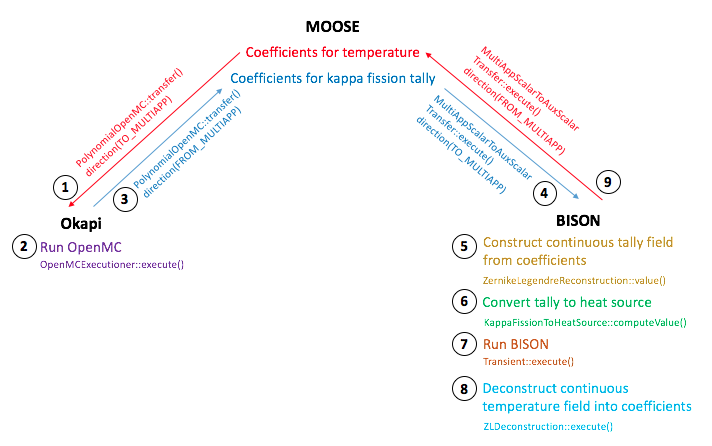
\includegraphics[width=15cm]{figures/OpenMC-BISON-complicated.png}
\end{figure}

\subsection{Nek and BISON Coupling}
This section discusses the coupling between Nek and BISON, where Nek is wrapped as a Moose App (MOON) to facilitate this coupling. The coupling discussed in this section was performed as a joint effort between INL and ANL in the fall of 2016.

\subsection{OpenMC, Nek, and BISON Coupling}
When coupling more than two applications using the MOOSE framework, there are several options for the coupling structure. In order to motivate the structure selected, an understanding of the limitations of the MOOSE coupling framework must be understood. The general coupling framework for a MOOSE simulation consists of a Master App and MultiApps. For each time step, unless sub-cycling is turned on (in which case one of the Apps may run at finer time steps than the others), all of the Apps, including the Master App, will execute. The order in which the execution of the Apps occurs is controlled with the {\tt execute\_on} parameter, which can take several values, most commonly {\tt timestep\_begin} and {\tt timestep\_end}. The MultiApps that execute on the start of a time step and on the end of a time step bound the execution of the Master App. If there are more than two MultiApps to a Master App, then in order to ensure full exchange of information at each time step, a custom routine for transferring data {\it in time} (not a custom {\tt Transfer} class, to be discussed later) is required. This would require developing a custom {\tt MultiApp} class, which is where the execution in time is controlled (note that there are other options for the {\tt execute\_on} parameter, but they are related to the finite element solve, such as {\tt linear\_residual} - with an external code that is not running any MOOSE kernels, these options don't make sense).

To keep the coupling as simple as possible and to avoid the need to develop custom Multi Apps (which is more intensive than developing custom transfers, executioners, and time steppers), the coupling is chosen to be limited to two distinct MultiApps per Master App. Note that this does {\it not} limit a total of two MultiApps per Master App - if the MultiApps are BISON and MOON, there may be many parallel instances of BISON, so long as there are only two distinct MultiApps (BISON and MOON). When selecting the Master App, the Master App can either perform a solve (and hence be one of Okapi, BISON, or MOON) or simply exist to transfer data between the Multi Apps (and hence be one of Okapi, BISON, MOON, PRONGHORN, RATTLESNAKE, etc. - the animal itself doesn't matter because it's only using capabilities in the MOOSE framework, not any physics-specific capabilities). The complication with using a master App for this three-way coupling that does not perform any physics solve is that it becomes much more difficult to control the execution of three peer Apps. There are only two available execution instructions that apply for non-MOOSE codes - {\tt timestep\_begin} and {\tt timestep\_end}, which does not offer enough flexibility in specification to define how {\it three} peer Apps should run.

If we restrict ourselves to only using two peer MultiApps per Master App, then the Master App must perform a physical solve. For a Master App that performs a physical solve, either BISON, MOON, or Okapi can be the Master App. Because multiple fuel pins can be simulated entirely in parallel (since a boundary coupling is employed with Nek), it would be inadvisable to have BISON be the Master App. This would restrict the coupling to a single fuel pin because there can only be a single Master App. A non-trivial amount of MPI code {\it could} allow this configuration to work correctly, but it would be much easier for either Okapi or MOON to be the Master App. 

The choice between MOON and Okapi for the Master App is more arbitrary than the choice to not choose BISON as the Master App, but is still based on characteristics of the coupling. Because Okapi is the only App that will solve for the entire domain (MOON solves in the fluid, BISON solves in the fuel), it is logical to choose Okapi as the Master App. The Okapi Master App both performs its own solve and transfers data between BISON and MOON. The example in {\tt tests/transfers/okapi-bison-nek} shows a functioning three-way coupling for a single fuel pin using this coupling structure. The figures that follow make references to variables in these files for the purpose of being explicit. The figure below shows all of the necessary methods to perform a three-way coupled simulation, with numbers indicating the order in which they would occur for a single Picard step. MOON is arbitrarily chosen to run first. 

\begin{figure}[H]
\centering
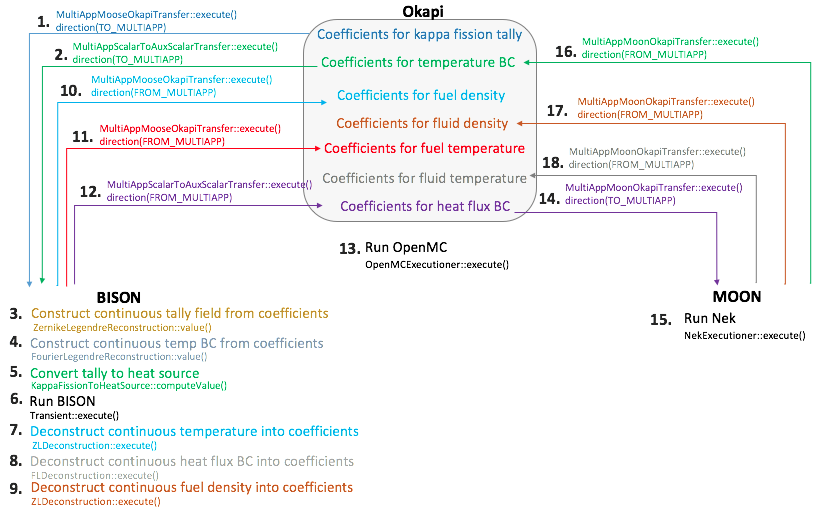
\includegraphics[width=17.5cm]{figures/OpenMC-BISON-Nek-complicated.png}
\caption{Sequence of events taken in one Picard iteration with MOON arbitrarily chosen to run first.}
\end{figure}

With Okapi as the Master App, either BISON can be run before MOON, or MOON run before BISON. Section \ref{sec:ICs} will discuss how boundary conditions are set based on which of the MultiApps executes first. For either choice of App running at the beginning of a time step versus at the end of a time step, the sequence of events is as follows. For MOON executing first, the following sequence of events occurs. To be as explicit as possible, refer to the working three-way example contained in {\tt okapi/tests/transfers/okapi-moose-nek} and {\tt moon/examples/okapi-moose-nek}. The following expansion orders are used in these files:

\begin{itemize}
\item Fourier order 5 (6 Fourier polynomials, so the Nek variable {\tt m\_fourier} equals 6) and Legendre order 10 (11 Legendre polynomials, so the Nek variable {\tt n\_legendre} equals 11) for transfer of surface heat flux and surface temperature conditions between Nek and BISON
\item Legendre order 0 (1 Legendre polynomial) and Zernike order 5 (21 Zernike polynomials)
\end{itemize}

\begin{enumerate}
\item Initialize the Master App. The actions performed here are generally the same regardless of which App is the Master App (i.e. this is not the stage at which the OpenMC input XML files would be read), since this purely sets up the entire MOOSE simulation by initializing MPI, allocating storage, etc. 
	\begin{enumerate}
	\item Set any initial conditions set in the Master App file. For MOON executing first, this sets an initial condition on the heat flux that is passed from Okapi to MOON (since BISON has not yet run). A dummy value of 1.0 is used for the initial condition (for the zero-th order component).
	\end{enumerate}
\item Initialize MOON. This sets initial conditions specified in the MOON input file and {\it then} calls the {\tt NekExecutioner::init()} method (because we call the {\tt init()} method of {\tt Transient} before that of {\tt NekExecutioner}) and reads Nek input files to perform internal actions such as setting initial values. 
\item Initialize BISON. This calls the initialization method of the executioner specified in the BISON input file. This is where initial conditions set in the BISON input file are set.
%
\item Initialize the Master App. This step is not redundant with step 1, but rather this calls the {\tt init()} method of the {\tt OpenMCExecutioner}, which reads OpenMC input files and performs internal actions such as setting initial values that are defined in the OpenMC input files.
%
\item Execute all transfers on {\tt timestep\_begin} with direction {\tt to\_multiapp}.
	\begin{enumerate}
	\item Transfer heat flux boundary condition coefficients from Okapi to MOON. For the very first time step none of the Apps have been run yet, so an initial condition must be specified on the heat flux boundary condition in the master input file.
	\end{enumerate}
\item Solve Nek.
\item Execute all transfers on {\tt timestep\_begin} with direction {\tt from\_multiapp}.
	\begin{enumerate}
	\item Transfer temperature boundary condition coefficients from MOON to Okapi. For the very first Nek step, the temperature boundary coefficients are all computed to be zero (this does not impact Okapi because it doesn't use the temperature boundary conditions).
	\item Transfer axially-binned values for fluid density and temperature from Nek to Okapi (not yet implemented).
	\end{enumerate}
\item Solve Okapi.
\item Execute all transfers on {\tt timestep\_end} with direction {\tt to\_multiapp}.
	\begin{enumerate}
	\item Transfer kappa fission distribution coefficients from Okapi to BISON.
	\item Transfer temperature boundary condition coefficients from Okapi to BISON (for the very first time step, these coefficients are all zero because Nek computes them as so).
	\end{enumerate}
\item Solve BISON.
\item Execute all transfers on {\tt timestep\_end} with direction {\tt from\_multiapp}.
	\begin{enumerate}
	\item Transfer fuel temperature coefficients from BISON to Okapi.
	\item Transfer fuel density coefficients from BISON to Okapi (not yet implemented).
	\end{enumerate}
\end{enumerate}

And for BISON executing first, the sequence of events are similar, except that steps 5-7 dealing with MOON execution and transfer are swapped with steps 9-11 dealing with BISON execution and transfer. With MOON executing before BISON, the following figure shows all of the steps taken for the very first Picard step, which shows where the initial conditions come from and how variables in each of the three codes interact. For all of the subsequent time steps, the ``initial conditions'' simply become the values computed from the last time step. Note that the data transfer for fuel density and fluid density and temperature are not shown because they are not yet implemented.

\begin{figure}[H]
\centering
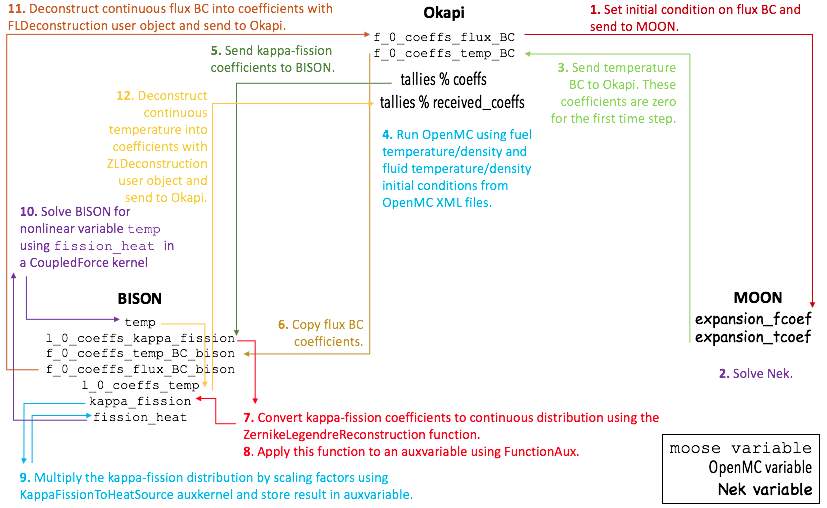
\includegraphics[width=17.5cm]{figures/OpenMC-BISON-Nek-step1.png}
\caption{Sequence of events and variables used to store coupling data for the three-way OpenMC, BISON, and Nek coupling. The fonts used for different variables are shown in the box in the lower right.}
\end{figure}

\clearpage
\section{Initial Conditions}
\label{sec:ICs}
This section discusses how initial conditions are applied to OpenMC, Nek, and BISON for a coupled solve. There are generally two types of initializations that are performed for a single physics code:

\begin{itemize}
\item Initializations that specify the geometry, materials, and problem parameters that will remain unchanged throughout a simulation
\item Initial values for solution variables that are needed to begin the finite difference time marching
\end{itemize}

It becomes increasingly difficult as the number of coupled codes increases to ensure consistency between all of the initial conditions and system specifications. To attempt to achieve consistency, all initial conditions should be set from MOOSE. However, if desired, these MOOSE initial conditions can be omitted, and initial conditions can be set in the usual manner in the code's input files (OpenMC's XML files or Nek's {\tt rea} and {\tt usr} files). Either MOON or Buffalo may execute first, so the required initial conditions depends on this choice. Note that the requirements to set boundary conditions also depends on the extent to which the transfer classes have been completed - if the capability to transfer fluid density has not yet been implemented in Nek, for example, then an initial condition must be specified on the fluid density for OpenMC. 

\subsection{MOON Before BISON}
When MOON runs before BISON, initial conditions must be specified for fields that are inputs to MOON and for those fields that are inputs to Okapi that would have been determined by BISON. The fields that must have initial conditions are:

\begin{itemize}
\item Heat flux boundary condition (BISON does not run before Nek)
\item Fluid-specific boundary conditions that are required by Nek, such as fluid inlet temperature/density, pressure, etc. These type of boundary conditions vary depending on the problem specifics.
\item Fuel density (BISON does not run before OpenMC)
\item Fuel temperature (BISON does not run before OpenMC)
\end{itemize}

\subsection{BISON Before MOON}
When BISON runs before MOON, initial conditions must be specified for fields that are inputs to BISON and for those fields that are inputs to Okapi that would have been determined by Nek. This section discusses how to set these initial conditions. These fields that must have initial conditions are:

\begin{itemize}
\item Kappa-fission distribution (OpenMC does not run before BISON)
\item Temperature boundary condition (Nek does not run before BISON)
\item Fluid density (Nek does not run before OpenMC)
\item Fluid temperature (Nek does not run before OpenMC)
\end{itemize}

\clearpage
\section{Data Transfer}
This section first discusses the general requirements needed to transfer information between two physics codes. Then, subsections focusing on MOOSE, OpenMC, and Nek will individually describe the data transfer capabilities introduced in order to transfer information between all three codes. When coupling two codes, there are two general ways in which the data can be transferred:

\begin{enumerate}
\item Force both codes to solve on the same mesh, in which case the data transfer can be accomplished by determining a functional form for the transfer variable (such as temperature) over a single computational element, and then passing this information to the second code. Assuming that the second code can utilize this information exactly, this is the easiest way to transfer information, because it requires little effort to map cells in one mesh to cells in another. However, this method is very restrictive, since it is often the case that the two physics do not require the same mesh, and forcing both physics to run on the finest mesh is unnecessarily expensive. For instance, boundary layers must be resolved for fluids computations with very fine elements that would be overkill for a Monte Carlo simulation. When one of the codes is a meshless code, such as Monte Carlo codes using Constructive Solid Geometry representations, this ``easiness'' is no longer present.
\item Run both codes on different meshes.

	\begin{enumerate}
	\item Use arbitrary polynomials to express a transfer variable, and then pass the expansion coefficients to the second code. For instance, suppose Nek is to transfer temperature on a boundary to MOOSE, which would use this information to set a boundary condition. Because this information is not being passed on an element-to-element basis, its spatial distribution must be described using some type of function - delta functions if an elementwise-constant value from Nek is to be transferred to an element (not necessarily of the same size) in MOOSE, or really any arbitrary polynomial. To transfer a variable \(u(r, \theta, z)\) to MOOSE, Nek would compute the expansion coefficients \(C_{jkl}\) that capture the behavior according to expansion functions \(R(r), \Theta(\theta), Z(z)\):
	
	\beq
	\label{eq:GenericExpansion}
	u(r, \theta, z)\approx\sum_{j=0}^J\sum_{k=0}^K\sum_{l=0}^L C_{jkl}R_j(r)\Theta_k(\theta)Z_l(z)
	\eeq
	
Note that an approximate equals sign \(\approx\) is used, since for an arbitrary selection of functions, the (potentially) infinite degrees of freedom of the value of \(u\) computed by Nek cannot be fully captured. Once Nek passes the coefficients \(C_{jkl}\) to MOOSE, MOOSE would reconstruct the functional form of the transfer variable using the same equation above, and then proceed with its simulation for that step. The issue with using arbitrary polynomials is that there is no one way to determine the expansion coefficients \(C_{jk}\). For instance, assume we use the following expansion functions:

	\beqa
	R_j(r)=&r^j\\
	\Theta_k(\theta)=&\cos(k\theta)\\
	Z_l(z)=&1+z^l\\
	\eeqa

To determine the expansion coefficients for this choice requires that we construct a Vandermonde matrix, which requires that we arbitrarily select points over the Nek element at which to sample the Nek transfer variable. For \(J=1\), \(K=0\), \(L=0\), this matrix system would take the form:

\beqa
u(r,\theta,z)=\begin{bmatrix}
r_0^0\cos{(0)}(1+z_0^0) & r_0^1\cos{(\theta_0)}(1+z_0^0)\\
r_1^0\cos{(0)}(1+z_0^0) & r_1^1\cos{(\theta_0)}(1+z_0^0)\\
\end{bmatrix}
\begin{bmatrix}
C_{000}\\C_{100}
\end{bmatrix}
\eeqa

where \(r_0\) and \(r_1\) are the two sampled \(r\)-coordinates in the element that must be selected in order to determine the expansion coefficients for a first-order \(r\)-expansion, and \(\theta_0\) and \(z_0\) the sampling points to determine the expansion coefficients for a zeroth-order \(\theta\)- and \(z\)-expansion. This can cause problems such as oscillations in the interpolation if the choices of functions are poor, and can completely miss parts of the transfer variable solution if we happen to not select points near important features. In addition, if we use a statistical code such as a Monte Carlo code, choosing these sampling points will make any scores to other regions of the problem completely ``useless,'' which will lead to very high numbers of particles required to reduce variance.

	\item Use orthogonal functions to express a transfer variable, and then pass the expansion coefficients to the second code. Using orthogonal functions is essentially the same formulation as that shown in Eq. \eqref{eq:GenericExpansion}, except that the expansion functions are chosen to be orthogonal over the domain of transfer. Then, orthogonality conditions lead to exact formulas for \(C_{jkl}\) that are {\it integral} in nature, which means that all features of the solution are captured, and no creation and inversion of a Vandermonde matrix is required. 
	\end{enumerate}
	
\end{enumerate}

For the reasons discussed above, the data transfer between OpenMC, Nek, and BISON is performed using orthogonal polynomial expansions. For any code to implement data transfers using polynomials, four capabilities are required:

\begin{enumerate}
\item Functions to compute the orthogonal polynomials given a coordinate point and expansion order.
\item Routines to integrate a continuous variable over an orthogonal domain to compute the expansion coefficients. This process will be referred to in this document as ``deconstruction,'' since a continuous field is decomposed into a finite set of expansion coefficients.
\item Routines to multiply a set of expansion coefficients by orthogonal polynomials to form a continuous field form a set of finite coefficients. This process will be referred to in this document as ``construction,'' since a continuous field is formed from a set of discrete expansion coefficients.
\item Use the constructed field in some internal capacity that defines the coupling, such as in the specification of a boundary condition or heat source.
\end{enumerate}

After a summary of orthogonal polynomials available, each of these four capabilities will be described in detail for MOOSE, OpenMC, and Nek. 

\subsection{Choices of Orthogonal Polynomials}
\label{sec:Polynomials}
This section describes several choices of orthogonal polynomials that can be used to construct and deconstruct continuous fields.

\subsubsection{Legendre Polynomials}

Legendre polynomials are orthogonal over \( -1 \leq z \leq 1\), and hence are suitable for expanding solutions along the axes of fuel pins, along one direction in a slab, or in any Cartesian dimension. The Legendre polynomials are given as:

\beq
\label{eq:LegendreScaled}
P_l(z)=\sqrt{\frac{2l+1}{2}}\frac{1}{2^ll!}\frac{d^l}{dx^l}\left\lbrack\left(z^2-1)^l\right)\right\rbrack
\eeq

which are orthogonal over \(-1\) to \(+1\):

\beq
\label{eq:LegendreScaledOrthogonality}
\int_{-1}^{+1}P_l(z)P_{l'}(z)dz=\delta_{ll'}
\eeq

\subsubsection{Fourier Polynomials}

Fourier polynomials are orthogonal over \(-\pi\leq\theta\leq\pi\), and hence are suitable for expanding along the \(\theta\) direction of a cylinder. The Fourier functions are given as:

\beq
\label{eq:FourierScaled}
F_k(\theta)=
\begin{cases}
\frac{1}{\sqrt{\pi}}\cos{(k\theta)} & k \neq 0\\
\frac{1}{\sqrt{2\pi}}\cos{(k\theta)} & k = 0\\
\end{cases}
\eeq

which are orthogonal over \(-\pi\) to \(+\pi\):

\beqa
\label{eq:FourierOrthogonal}
\int_{-\pi}^{+\pi}F_k(\theta)F_{k'}(\theta)d\theta=\delta_{kk'}
\eeqa

\subsubsection{Zernike Polynomials}

Zernike polynomials are orthogonal over the unit circle, and hence are suitable for expanding in the plane of a cylinder. The Zernike polynomials are given as:

\beq
\label{eq:ZernikeScaled}
Z_n^m(r,\theta)=
\begin{cases}
\sqrt{\frac{2(n+1)}{\pi\left(1+\delta_{m0}\right)}}R_n^{|m|}(r)\cos{(m\theta)} & m\geq 0\\
-\sqrt{\frac{2(n+1)}{\pi\left(1+\delta_{m0}\right)}}R_n^{|m|}(r)\sin{(m\theta)} & m < 0\\
\end{cases}
\eeq

\beq
R_n^{|m|}(r)=\sum_{s=0}^{\frac{n-|m|}{2}}\frac{(-1)^s(n-s)!}{s!\left(\frac{n+|m|}{2}-s\right)!\left(\frac{n-|m|}{2}-s\right)!}r^{n-2s}
\eeq

Note that \(m\) can only obtain values \(-n, -n+2, -n+4, \cdots, n\). The orthogonality condition is:

\beq
\label{eq:ZernikeOrthogonal}
\int_{0}^{1}rdr\int_{0}^{2\pi}d\theta Z_{n}^m(r,\theta)Z_{n'}^{m'}=\delta_{n,n'}\delta_{m,m'}
\eeq

\subsection{Deconstructing a Continuous Variable}
This section describes how a continuous field \(u(r,\theta,z)\) can be deconstructed into a set of expansion coefficients using orthogonal polynomials. The procedure is the same regardless of the orthogonal domain (i.e. if performing a boundary or volume coupling), but will be illustrated for both a boundary coupling over the surface of a cylinder and for a volume coupling over a cylindrical volume. For a boundary coupling over the surface of a cylinder, a function \(u(\theta,z)\) can be expressed as:

\beq
\label{eq:OrthogonalExpansion}
u(\theta, z)\approx\sum_{k=0}^K\sum_{l=0}^LC_{kl}F_k(\theta)P_l(z)
\eeq

where \(F_k(\theta)\) is the \(k\)-th order Fourier function and \(P_l(z)\) is the \(l\)-th order Legendre polynomial. The expansion coefficients can be determined by multiplying both sides of Eq. \eqref{eq:OrthogonalExpansion} by orthogonal polynomials of different order, and applying the orthogonality conditions given in Section \ref{sec:Polynomials}:

\beq
\label{eq:ScaledExpansionCoeff}
C_{kl}=\int_{-1}^{+1}dz\int_{-\pi}^{+\pi}d\theta u(\theta, z)F_k(\theta)P_l(z)
\eeq

Likewise, for a volume coupling over a cylinder, a function \(u(r,\theta,z)\) can be expressed as:

\beq
\label{eq:ZLReconstruction}
u(r,\theta,z)=\sum_{l=0}^{L}\sum_{n=0}^N\sum_{m=-n}^{n}C_{l}^{nm}P_l(z)Z_n^m(r,\theta)
\eeq

Again, the coefficients can be determined by multiplying by orthogonal polynomials of different order, and applying orthogonality conditions:

\beq
\label{eq:ZernikeLegendreCoefficient}
C_l^{nm}=\int_0^1rdr\int_{0}^{2\pi}d\theta\int_{-1}^{1}dzu(r,\theta,z)P_l(z)Z_n^m(r,\theta)
\eeq

Hence, all that is required to deconstruct a continuous field into a set of expansion coefficients is to perform repeated integrations over the orthogonal domain.

\subsection{Constructing a Continuous Variable}
As opposed to deconstruction, constructing a continuous variable from a set of expansion coefficients is more straightforward, since all that is required is repeated evaluation of the orthogonal polynomials, multiplied by expansion coefficients.

\subsection{MOOSE Data Transfer}
This section describes the capabilities introduced into the MOOSE source code that allows evaluation of polynomials, and construction/deconstruction of continuous fields. These functions are placed in a local branch of MOOSE so that BISON, Okapi, and MOON can all access these functions. The remote version of this special coupling version of MOOSE is located at {\tt git@github.com:aprilnovak/coupling-moose.git}.

\subsubsection{Evaluation of Polynomials}
This section discusses the generic functions added to MOOSE to compute orthogonal polynomials. MOON previously had several of these functions in its own source - to avoid duplication when other MOOSE animals require the access to the same functions, the {\tt LegendrePolynomial} and {\tt FourierPolynomial} functions were moved from MOON to MOOSE.

\color{magenta}
No checks are made that any of the normalizing parameters specified as input for these functions match those in external coupled codes.
\color{black}

\subsubsubsection{{\tt LegendrePolynomial}}
This function computes the Legendre polynomial in Eq. \eqref{eq:LegendreScaled} for a given value of \(l\) and a specific position. Because Legendre polynomials are only orthogonal on \([-1, +1]\), a scaling factor \(z\) is used to simply stretch or compress the physical domain to the orthogonal domain. The {\tt l\_geom\_norm} parameter provides the minimum and maximum distances over which the Legendre polynomials will be forced to be orthogonal using a scaling factor. 

\subsubsubsection{{\tt FourierPolynomial}}
This function computes the Fourier function given in Eq. \eqref{eq:FourierScaled} for a given value of \(k\) and a specific position. The \(\theta\) value at which to evaluate this function is determined as the angle between the two provided points. The user must provide the center of the circle for correct normalization. Because the fuel rod of interest for coupling exists on \([-\pi, +\pi]\), no additional scaling is needed.

\subsubsubsection{{\tt ZernikePolynomial}}
This function computes a Zernike polynomial given in Eq. \eqref{eq:ZernikeScaled} given orders \(n\) and \(m\). 

\subsubsection{Field Deconstruction}
This section describes how a continuous field is deconstructed into a set of expansion coefficients in MOOSE.

\subsubsubsection{{\tt FourierLegendreDeconstruction}}
This user object converts a continuous variable into the set of expansion coefficients that would be obtained by expanding the variable in Fourier and Legendre polynomials as shown in Eq. \eqref{eq:ScaledExpansionCoeff}. This user object only computes {\it one} \(C_{kl}\) coefficient at a time, so the {\tt FLDeconstruction} user object should be used instead, since it computes all the Legendre coefficients given a single Fourier order. Because the orthogonal domain likely differs from the physical domain, the actual integral performed is shown below:

\beq
C_{kl}=\frac{2}{RH}\int_{-1}^{+1}dz\int_{-\pi}^{+\pi}u(\theta, z)F_k(\theta)P_l(z)
\eeq

If both the numerator and denominator are multiplied by \(2\pi\), the denominator can be calculated using a surface area postprocessor. Note that this user object assumes that the coupled scalar auxvariable is organized by Fourier coefficient (each scalar auxvariable holds all the Fourier coefficients for a given Legendre order). 

Note that this user object {\it either} deconstructs a {\it scalar} variable \(u(\theta, z)\), {\it or} a vector-valued variable dotted with the unit normals, multiplied by a coefficient, \(-C\nabla u\cdot\hat{n}\) (since for coupling it is often desired to integrate a flux as well). The choice between these options is indicated with the {\tt flux\_integral} boolean parameter.

\color{magenta}
This user object will give inaccurate results if the integration is not performed over a cylindrical side surface, but no checks are made that the surface area matches the height and radius specified in the Fourier and Legendre polynomials.
\color{black}

\subsubsubsection{{\tt FLDeconstruction}}
This user object computes {\it all} of the Legendre coefficients given a fixed Fourier order, reducing the number of user objects required in the input file by a factor of the number of Legendre expansion coefficients. The contents of this user object are identical to that of the {\tt FourierLegendreDeconstruction} user object, except that loops are used to update an array of values instead of a singular value.

\color{magenta}
This user object will give inaccurate results if the integration is not performed over a cylindrical side surface, but no checks are made that the surface area matches the height and radius specified in the Fourier and Legendre polynomials.
\color{black}

\subsubsubsection{{\tt ZernikeLegendreDeconstruction}}
This user object converts a continuous variable into the set of expansion coefficients that would be obtained by expanding the variable in Zernike and Legendre polynomials as shown in Eq. \eqref{eq:ZernikeLegendreCoefficient}. This user object only computes {\it one} \(C_l^{nm}\) at a time, so the {\tt ZLDeconstruction} user object should be used instead, since it computes all of the Zernike coefficients given a single Legendre order. Because the orthogonal domain likely differs from the physical domain, the actual integral performed is shown below:

\beq
C_l^{nm}=\frac{1}{R^2}\frac{2}{H}\int_0^1rdr\int_{0}^{2\pi}d\theta\int_{-1}^{1}dzu(r,\theta,z)P_l(z)Z_n^m(r,\theta)
\eeq

where \(R\) is the radius and \(H\) the height in the physical domain. The factor of 2 appears because the height in the orthogonal domain is 2. By multiplying the factor above by \(\pi/\pi\), the denominator becomes the volume of the region. Hence, a postprocessor value provides the volume instead of relying on input from the user. This object can be restricted to blocks using the {\tt blocks} parameter in the input file. If the block is not specified, then if a variable parameter is present, the blocks are set to all of the blocks that are associated with that variable (i.e. for most simulations, the entire domain). If no variable is specified, then by default the entire domain is used. 

\color{magenta}
No checks are made to ensure that the integration is performed over a cylindrical domain. Results will be inaccurate if the domain is not cylindrical or if the provided functions are not given the same normalization quantities that are implicit in the provided domain. This could be improved by adding a check that the volume computed by the postprocessor matches the volume as-computed by the coupled Legendre and Zernike functions.
\color{black}

\subsubsubsection{{\tt ZLDeconstruction}}
This user object computes {\it all} of the Zernike coefficients given a fixed Legendre order, reducing the number of user objects required in the input file by a factor of the number of Zernike expansion coefficients. The contents of this user object are identical to that of the {\tt ZernikeLegendreDeconstruction} user object, except that loops are used to update an array of values instead of a singular value.

\color{magenta}
No checks are made to ensure that the integration is performed over a cylindrical domain. Results will be inaccurate if the domain is not cylindrical or if the provided functions are not given the same normalization quantities that are implicit in the provided domain. This could be improved by adding a check that the volume computed by the postprocessor matches the volume as-computed by the coupled Legendre and Zernike functions.
\color{black}

\subsubsection{Field Reconstruction}
This section discusses the functions developed in MOOSE to reconstruct a continuous field given expansion coefficients and specified orthogonal functions.

\subsubsubsection{{\tt FourierLegendreReconstruction}}
This function reconstructs a solution as a finite series of Fourier and Legendre polynomials given expansion coefficients, and evaluates it at a single point according to Eq. \eqref{eq:OrthogonalExpansion}. This function is set up so that the {\tt poly\_coeffs} coupled to this function {\it each} hold all of the expansion coefficients for a {\it fixed} Fourier order \(f\). For instance, for a Legendre expansion of 4 and a Fourier expansion of 2, these coefficients hold:

\begin{lstlisting}
f_0_coeffs = 'C00 C01 C02 C03 C04 C05'
f_1_coeffs = 'C10 C11 C12 C13 C14 C15'
f_2_coeffs = 'C20 C21 C22 C23 C24 C25'
\end{lstlisting}

where the first index represents the \(f\) order and the second the \(n\) order. Note that the choice in MOON was for each of these aux variables to hold all of the Legendre coefficients for a given Fourier order.

\subsubsubsection{{\tt ZernikeLegendreReconstruction}}
This function reconstructs a solution as a finite series of Zernike and Legendre polynomials given expansion coefficients, and evaluates it at a single point according to Eq. \eqref{eq:ZLReconstruction}. This function is very similar to the Fourier-Legendre reconstruction function developed for MOON, except that it also includes the flexibility for the Legendre expansion direction to not be along the \(z\)-direction. This function is set up so that the {\tt poly\_coeffs} coupled to this function {\it each} hold all of the expansion coefficients for a {\it fixed} Legendre order \(l\). For instance, for a Legendre expansion of 3 and a Zernike expansion of 2, these coefficients hold:

\begin{lstlisting}
l_0_coeffs = 'C000 C01n1 C011 C02n2 C020 C022'
l_1_coeffs = 'C100 C11n1 C111 C12n2 C120 C122'
l_2_coeffs = 'C200 C21n1 C211 C22n2 C2020 C222'
l_3_coeffs = 'C300 C31n1 C311 C32n2 C320 C322'
\end{lstlisting}

where the first index represents the \(l\) order, the second the \(n\) order, and the third the \(m\) order, where {\tt n} represents a negative number. Note that the choice in MOON was for each of these aux variables to hold all of the Legendre coefficients for a given Fourier order, which is the opposite of the choice here. 

\subsubsection{Using the Constructed Field}
This section discusses the capabilities added to MOOSE to use the constructed field to enact physical feedback with other physics.

\subsubsubsection{{\tt KappaFissionToHeatSource}}
OpenMC provides a set of kappa fission expansion coefficients to MOOSE. In order to use those coefficients, they must be converted to a heat source with units of W/volume (the FE mesh is units-agnostic). The {\tt ZernikeLegendreReconstruction} is used to expand these coefficients into a continuous distribution, and then the {\tt KappaFissionToHeatSource} auxkernel converts the continuous tally distribution to a heat source. There are two general methods by which to do this, both of which assume the user has knowledge of the power of the expansion domain. The power of the reactor is the sum of the power produced by fission directly in the fuel rod and the power produced by gamma heating (fuel, structural materials, and coolant). The expansion coefficients record the recoverable energy produced from {\it fission}, and hence will only have nonzero values over the fuel. So, assuming the user knows the power produced in each domain over which expansion coefficients are defined (a fuel pin, for example), the heat source can be determined by: 

\begin{itemize}
\item Multiplying the kappa fission distribution \(\kappa(\bf{r})\) (eV/source particle) by the user-specified pin fission power, divided by the integrated kappa fission distribution (over the pin):

\beq
\textrm{fission power}=\kappa(\bf{r})\times\frac{\textrm{user-defined pin fission power}}{\int d\bf{r}\kappa({\bf r})}
\eeq

\item Assuming an average energy released per fission \(E_f\) and an average number of source particles born from fission \(\nu\), the fission power may be computed as:

\beq
\textrm{fission power}=\kappa(\bf{r})\times\textrm{user-defined pin fission power}\times\frac{\nu}{E_f\int d\textbf{r}}
\eeq
\end{itemize}

The first approach is more desirable and general because it requires less assumptions than the second method (i.e. no assumptions are needed for values for \(\nu\) and \(E_f\)). However, for subtle reasons, the second method must be selected unless more changes are made to the MOOSE framework. After receiving expansion coefficients for the expansion coefficients from Okapi, BISON converts those just-received coefficients into a continuous distribution using the {\tt ZernikeLegendreReconstruction} function {\it simultaneously} with the application of the functional distribution to the continuous kappa-fission distribution auxiliary variable. The second method above requires that the auxiliary variable be fully constructed before integrating it, but this integrated value is required itself in the auxkernel that defines the auxvariable. This {\it could} be circumvented by setting an initial condition for the kappa-fisison coefficients in the BISON input file, which would be used to provide the postprocessor value for the first time step; all further time steps would lag one step in the value of the integrated kappa fission distribution. For early iterations, this lagging is undesirable, since there may be large changes in the kappa fission coefficients from one iteration to the next. Alternatively, if the second method is chosen, then the postprocessor is not required at all, at the expense of slight inaccuracies in the assumption of constant \(\nu\) and \(E_f\).

This kernel requires the user to input the initial steady state power. A one-delayed neutron group approximation can then be used to account for (very approximate) changes in power due to thermal-hydraulic feedback. It is customary to group the delayed neutron precursors into six groups, but if the delayed neutron precursors are bundled into a single group, then the point kinetics equations become considerably simpler:

\beq
\label{eq:PointKineticsPrecursor_OneDelayedGroup}
\frac{\partial C(t)}{\partial t}=\frac{\beta}{\Lambda}n(t)-\lambda C(t)
\eeq

\beq
\label{eq:PointKineticsNeutrons_OneDelayedGroup}
\frac{\partial n(t)}{\partial t}=\left\lbrack\frac{\rho(t)-\beta}{\Lambda}\right\rbrack n(t)+\lambda C(t)
\eeq

where \(\lambda\) represents a decay constant that is weighted by all of the precursor groups:

\beq
\label{eq:Lambda_OneGroup}
\lambda=\left(\frac{1}{\beta}\sum_{i=1}^{6}\frac{\beta_i}{\lambda_i}\right)^{-1}
\eeq

and \(\beta\) is now the sum of all of the \(\beta_i\) for each precursor group:

\beq
\beta=\sum_{i}\beta_i
\eeq

and \(\Lambda\) is the effective neutron generation time. To solve Eqs. \ref{eq:PointKineticsPrecursor_OneDelayedGroup} and \ref{eq:PointKineticsNeutrons_OneDelayedGroup}, we need two initial conditions. These initial conditions can be obtained by assuming that at \(t=0\) the reactor was at steady state such that the time derivatives are zero:

\beqa
\label{eq:PKE_OneGroup_ICs}
n(t=0)=&\ n_0\\
C(t=0)=&\frac{\beta}{\lambda\Lambda}n_0\\
\eeqa

This system of equations can be solved by seeking exponential solutions of the form \(n=n\exp(\omega t)\) and \(C=C\exp(\omega t)\). Note that this essentially implies that the frequency of the neutron population and the precursor population are the same, which is as expected with a single delayed neutron group. Inserting these forms into Eqs. \ref{eq:PointKineticsPrecursor_OneDelayedGroup} and \ref{eq:PointKineticsNeutrons_OneDelayedGroup} and canceling the exponential terms, we obtain:

\beqa
\label{eq:PKE_OneGroup_AssumedForm}
C\omega=&-\lambda C+\frac{\beta}{\Lambda}n\\
n\omega=&\lambda C+\left(\frac{\rho(t)-\beta}{\Lambda}\right)n\\
\eeqa

Substituting \(C\) from the first equation into the second gives two solutions for \(\omega\):  

\beq
\label{eq:PKEomega}
\omega=\frac{-(\Lambda\lambda+\beta-\rho)\pm\sqrt{(\Lambda\lambda+\beta-\rho)^2+4\Lambda\lambda\rho}}{2\Lambda}
\eeq

Hence, because we have two solutions for \(\omega\), our solutions are of the form:

\beqa
\label{eq:PKE_Solutions_OneGroup}
n(t)=&n_1\exp{\omega_1 t}+n_2\exp{\omega_2 t}\\
C(t)=&C_1\exp{\omega_1 t}+C_2\exp{\omega_2 t}\\
\eeqa 

Using our two initial conditions from Eq. \ref{eq:PKE_OneGroup_ICs} and by plugging in the solutions into the original differential equations (to obtain two time-dependent conditions) in Eqs. \ref{eq:PointKineticsPrecursor_OneDelayedGroup} and \ref{eq:PointKineticsNeutrons_OneDelayedGroup} will provide four equations and four unknowns (\(P_1, P_2, C_1, C_2\)). The solution for neutron population then becomes:

\beq
\label{eq:PowerPKE}
n(t)=n_0\left(\frac{\omega_1+\lambda}{\lambda}\frac{\omega_2}{\omega_2-\omega_1}\exp{\omega_1 t} + \frac{\omega_2+\lambda}{\lambda}\frac{\omega_1}{\omega_1-\omega_2}\exp{\omega_2 t}\right)
\eeq

The two-term exponential behavior will give two different time behaviors, where the \(\omega_1\) term represents the prompt power jump that occurs due to a near-immediate change in the prompt neutron population. The \(\omega_2\) term, which will necessarily result in a slower time response since \(\omega_2<\omega_1\), represents the neutron population changes due to changes in the delayed neutron population. Eq. \eqref{eq:PowerPKE} is implemented in this kernel, where it is implicitly assumed that there is a direct relationship between neutron population \(n\) and power. The use of this model is optional.

The assumptions made in this one-delayed neutron group include all of the approximations that are also made in the diffusion equation (the flux is at most linearly anisotropic in angle and changes in current are much smaller than the magnitude of current), as well as:

\begin{itemize}
\item The system begins at steady state (\(k=1\))
\item There is only one delayed neutron group
\item The flux is separable in both space and time, and the spatial dependence is given by the first eigenfunction to the diffusion equation (characterized by the geometric buckling)
\item The delayed neutron precursor distribution can be described the same spatial distribution as the neutron population
\end{itemize}

\subsubsection{Performing the Data Transfer}
This section describes the MOOSE transfer classes developed to transfer data between Okapi and BISON and Okapi and MOON; because Okapi is the Master App, BISON and MOON do not communicate with each other directly. The OpenMC and Nek routines that are called from within the MOOSE transfer classes developed are discussed in Sections \ref{sec:OpenMCTransfer} and \ref{sec:NekTransfer}, respectively. The convention for naming these transfer classes is the name of the sub App followed by the name of the Master App (the {\tt MultiAppMooseOkapiTransfer} class is used to transfer data between MOOSE and Okapi when MOOSE is the sub App to an Okapi Master App). This distinction is required because slightly different syntax is required for obtaining references to variables in the Master App versus Sub Apps. Note that this section is subject to change once the Functional Expansion MOOSE module is complete.

\subsubsubsection{{\tt MultiAppMooseOkapiTransfer}}
This transfer object defines data transfer from MOOSE to OpenMC (from MultiApp), and from OpenMC back to MOOSE (to MultiApp). In order to be flexible such that this transfer class can be used for both transfer to and from OpenMC, the {\tt to\_aux\_scalar} parameter will be a dummy parameter for transfer to OpenMC (because OpenMC does not perform any finite element solve in the MOOSE context), while {\tt source\_variable} will be a dummy variable for transfer from OpenMC for the same reason.
\\\\
{\it Transfer to OpenMC}\\
This transfer is used to pass coefficients for fuel temperature from MOOSE to OpenMC. The source variable holds a list of the scalar auxvariables that hold all of the expansion coefficients for a given Legendre order for the fuel temperature. These must be present in ascending Legendre order so that OpenMC interprets these coefficients correctly. These fuel temperature coefficients are stored in an array that is passed to the {\tt receive\_coeffs\_for\_cell} subroutine, which stores these coefficients in the {\tt t \% received\_coeffs} array. The total number of coefficients available is used to allocate this array if it has not yet been allocated, and for all transfers but the first, if the number of coefficients coming from MOOSE disagrees with the number from OpenMC, an error is thrown. Finally, the OpenMC subroutines that are called from {\tt MultiAppOkapiMooseTransfer} methods require the OpenMC cell index in the {\tt cells(:)} array so that we know which cells to change the temperature of. The following checks are in place:

\begin{itemize}
\item All of the source variables must be the same length
\item The OpenMC cell ID must be a valid cell
\item Number of coefficients from MOOSE must match the number from MOOSE that was used to allocate the size of the array
\end{itemize}

After OpenMC receives these coefficients, no routines are available yet to implement continuous temperature tracking, so the zeroth order coefficient is used to manually change the temperature by calling the {\tt openmc\_set\_cell\_temperature} subroutine directly from the transfer class. Note that to change a temperature in OpenMC requires that you have loaded cross sections at that temperature; a range of temperatures can be loaded during the initialization step by specifying the {\tt temperature\_range} parameter in the settings XML file.

\color{magenta}
This transfer only works for a single coupling cell, since we won't duplicate the transfer block shown below for every single fuel pin. We'll need to write some method to internally link the OpenMC cells with the MOOSE block IDs. A routine needs to be developed to receive the expansion coefficients in OpenMC, and store them as a function of the OpenMC cell to which they pertain. Finally, continuous material tracking needs to be implemented in OpenMC to make actual use of these coefficients.
\color{black}
\\\\
{\it Transfer to MOOSE}\\
For transferring data from OpenMC to MOOSE, the {\tt fet\_deconstruction} OpenMC subroutine is first called in order to collect all of the expansion coefficients into the {\tt coeffs(:, :)} array. The {\tt fet\_deconstruction} subroutine sums over all other filters except the cell filter. For instance, if the user specifies multiple material filters, the expansion coefficients are summed over all of those materials, simply returning coefficients by cell. The number of these expansion coefficients is defined based on the FETs that appear in the {\tt tallies.xml} file. In order to extract the expansion coefficients from OpenMC, the {\tt get\_coeffs\_from\_cell} OpenMC subroutine stores the expansion coefficients for a specified cell in a C++ array. The following checks are in place:

\begin{itemize}
\item All of the variables to write must be the same length
\item The total size of the variables to write must match the number of coefficients in OpenMC (this check is made in OpenMC by comparing with the size of the C++ array passed to the {\tt get\_coeffs\_from\_cell} subroutine). Because each of the variables must be the same length, and the total number of coefficients must match, this also ensures that the correct number of scalar aux variables are provided.
\item The OpenMC cell ID must be valid
\end{itemize}

\color{magenta}
Like the transfer to OpenMC, this transfer only works for a single fuel pin, and in the future we'll need to internally specify which OpenMC cells map to MOOSE blocks.
\color{black}

\subsubsubsection{{\tt MultiAppMooseOkapiReactivityTransfer}}
This transfer is used to transfer \(k_{eff}\) from Okapi to MOOSE for uses such as in point kinetics approximations that require knowledge of the system reactivity. This transfer is only defined for the direction of Okapi to MOOSE, since no reactivity can be transferred in the other direction. This transfer is separated from the {\tt MultiAppMooseOkapiTransfer} class for modularity.

\subsubsubsection{{\tt MultiAppMoonOkapiTransfer}}
This transfer object defines what routines are called to transfer data from Okapi to Nek, and from Nek back to Okapi. In order to be flexible such that the transfer can be used for both transfer to and from Nek, the {\tt to\_aux\_scalar} parameter will be a dummy parameter for transfer to Nek (because Nek does not perform any finite element solve in the MOOSE context), while {\tt source\_variable} will be a dummy variable for transfer from Nek for the same reason.
\\\\
{\it Transfer to Nek}\\
When transferring data from Okapi to Nek, the expansion coefficients are stored in the {\tt coeff\_fij} array that is the only member of the {\tt expansion\_fcoef\_} struct. {\tt expansion\_fcoef\_} represents the direct mapping of a Fortran common block to a C++ struct (note the trailing underscore). After writing to the flux expansion coefficient array, the {\tt flux\_reconstruction} subroutine is called, which reconstructs a continuous heat flux surface boundary condition. This transfer is used to pass all of the flux BC coefficients at once, where the aux scalar variables holding the coefficients must be listed in ascending Fourier order, where each scalar variable holds all of the Legendre coefficients for a fixed Fourier order. The following checks are in place:

\begin{itemize}
\item All of the scalar variables to read must be the same length
\item The number of scalar variables to read must match the {\tt m\_fourier} Nek variable
\item The length of each scalar variable to read must match the {\tt n\_legendre} Nek variable
\end{itemize}

{\it Transfer from Nek}\\
When transferring data from Nek to Okapi, the expansion coefficients from the {\tt coeff\_tij} array that is the only member of the {\tt expansion\_tcoef} common block are read and stored in an auxvariable in Okapi. This auxvariable serves as a ``middle-man'' for intermediate storage before being sent to BISON, where the information is eventually used. For this transfer of temperature BC coefficients, the following checks are in place:

\begin{itemize}
\item All of the scalar variables to write must be the same length
\item The number of scalar variables to write must match the {\tt m\_fourier} Nek variable
\item The length of each scalar variable to write must match the {\tt n\_legendre} Nek variable
\end{itemize} 

In addition, this transfer direction is used to change the temperatures of axial layers in the fluid based on volume integration that is performed in the {\tt axially\_binned\_integration} Nek subroutine. This requires a vector of OpenMC cell IDs to be provided, which are then used with the {\tt openmc\_cell\_set\_temperature} routine to change temperatures in OpenMC for cell layers. The following check is in place:

\begin{itemize}
\item The number of OpenMC cells provided must match the number of layers defined in Nek
\end{itemize}

\color{magenta} A current limitation is that the expansion orders for the heat flux and temperature boundary conditions are the same, but this is not a physical limitation. In addition, once continuous temperature tracking is implemented, there will no longer be a need for the user to specify the axial cells manually in the geometry XML file, and so the axial fluid temperature portion of this transfer will need to be modified.\color{black}

In addition to transferring expansion coefficients for a surface temperature boundary condition, the {\tt axially\_binned\_integration} Nek subroutine is called to integrate the fluid temperature and density and store axially-binned averages in the {\tt fluid\_temp\_bins} Nek array. No subroutines in OpenMC have been developed to utilize axially-binned averages of temperature.

\subsection{OpenMC Data Transfer}
\label{sec:OpenMCTransfer}
This section describes the capabilities introduced into the OpenMC source code that allow evaluation of polynomials, construction/deconstruction of continuous fields, and the use of this transferred data to enact physical changes, such as changing temperatures and densities. The information in this section is based upon the {\tt zernike} branch provided by Matt Ellis, and corrections and extensions that were made are indicated where applicable.

\subsubsection{Evaluation of Polynomials}
OpenMC contains several functions in the {\tt math} module to compute polynomial values given a coordinate and order, and in the {\tt tally} module to compute normalized positions. For evaluation of orthogonal polynomials, for performance no checks are made to ensure that the provided coordinates are within valid ranges, so use of normalize coordinates is required.

\subsubsubsection{{\tt calc\_pn(n, x)}}
\label{sec:calc_pn}
This function computes a Legendre polynomial given an order \(n\) and a coordinate \(x\), where this \(x\)-coordinate must be within the valid range \(-1\leq x\leq1\). This function provides Legendre polynomials up to order 10, beyond which a value of 1 is returned. This function does not compute the {\it scaled} Legendre polynomials that are needed for neat computation of expansion coefficients for an orthogonal expansion (they should be multiplied by \(\sqrt{(2l+1)/2}\)). 

\subsubsubsection{{\tt calc\_pn\_scaled(n, x)}}
This function computes the scaled Legendre polynomial that is needed for correctly computing FET expansion coefficients (without needing to worry about carrying the \(\sqrt{(2l+1)/2}\) coefficient around). This function simply calls the {\tt calc\_pn} subroutine, and hence suffers the same limitations as those discussed in Section \ref{sec:calc_pn} with regards to order and position checking. 

\subsubsubsection{{\tt calc\_zn(n, rho, phi)}}
\label{sec:calc_zn}
This function computes the Zernike polynomials for an order \(n\), radial coordinate \(\rho\), and angular coordinate \(\phi\) assuming that these coordinates have already been correctly scaled to the unit circle. For a given value of \(n\), the output of this function is an array \(zn\) of length \(n+1\), i.e. the output array holds all of the \(n=\) fixed, \(m\) values for the given \(n\). Similar to {\tt calc\_pn}, this function does not correctly scale the Zernike polynomials - they should all be divided by a factor of \(\sqrt{\pi}\) to ensure that integration over the orthogonal domain directly gives the expansion coefficients, without other factors trailing around. This routine computes the Zernike polynomials up to order 18.

\subsubsubsection{{\tt calc\_zn\_scaled(n, rho, phi)}}
This function computes the scaled Zernike polynomials that are needed for correctly computing FET expansion coefficients (without needing to worry about carrying the \(1/\sqrt{\pi}\) coefficient around). This function simply calls the {\tt calc\_zn} subroutine, and hence suffers the same limitations as those discussed in Section \ref{sec:calc_zn} with regards to order and position checking.

\subsubsubsection{{\tt get\_polynomial\_norm\_positions(...)}}
This subroutine obtains normalized coordinate positions to be used as input to the functions discussed above. This function computes normalized \(r, \theta, z\) coordinates, where the \(r, \theta\) coordinates are normalized to the unit circle and the \(z\) coordinate to the \([-1, 1]\) orthogonal domain for Legendre polynomials. The type of score passed into this routine determines which type of normalization is performed. This subroutine was extended from Matt's implementation by back-determining certain geometric information so that the user does not need to redundantly specify it in the input file. In addition, it was previously implicitly assumed that the geometry were centered on \(0, 0\) - this has been made more general. A particle is input to this subroutine, and the {\tt region} array for the particle's cell looped over until finding the surfaces that are \(z\)-cylinders and \(z\)-planes. From these surfaces, the cylinder center, radius, and axial distance between the \(z\)-planes is determined. Note that because only \(z\)-cylinders and surfaces are investigated, this limits the FETs to being defined in the \(z\)-direction. 

\color{magenta}
Additional improvements here would make this more general so that the expansion could be performed in any direction, and for any type of expansion tally (calculating normalized coordinates over a cylinder assumes we're using a Zernike-Legendre expansions).
\color{black}

\subsubsection{Field Deconstruction}
OpenMC deconstructs a statistical distribution of fission events into expansion coefficients for the fission source. Tallies are used to compute these expansion coefficients. A tally \(X\) at its most fundamental level can be described almost entirely by its score and filter(s). A filter represents the region of phase space over which to tally, and the score the ``what'' to tally. 

\beq
X=\underbrace{\int dE\int d\bf{r}\int d\hat{\Omega}\int dt}_{\textrm{filters}} \underbrace{f(E,\bf{r},\hat{\Omega},t)}_{\textrm{score}}\psi(E,\bf{r},\hat{\Omega},t)
\eeq

For coupling to an external code, a Monte Carlo code computes a fission power distribution (W/volume) in the fuel that is used by that external code to perform a simulation to determine an updated temperature. Deconstructing the fission power distribution into a set of expansion coefficients requires using tallies to compute the expansion coefficients. OpenMC already has the {\tt kappa-fission} tally, which computes the recoverable energy production due to fission. This energy includes the fission product kinetic energy, prompt and delayed neutron kinetic energies, prompt and delayed gamma ray energies, and the total energy released from \(\beta\) particles. Neutrino energies are assumed to not deposit in the system. The prompt and delayed gamma ray energy is assumed to deposit locally, so this tally would not provide any estimate of the fission energy deposition (by photons) directly in the coolant, since no fission will occur directly in the coolant (and OpenMC does not have photon transport capabilities, anyways). The units for this tally are eV per source particle, and with proper transformations, this can be converted to a fission power density. Note that the {\tt kappa-fission} tally (unlike the {\tt fission-q-recoverable} tally) does not use energy-dependent \(Q\)-values, but does use nuclide-dependent values. The {\tt kappa-fission} tally computes the score \(f\) for analog tallies as:

\beq
f=\sum_{i}w_iQ_i\frac{\sigma_{f,i}}{\sigma_{a,i}}\phi
\eeq

where if there is no survival biasing, then we need to skip scoring to this tally for all absorption events (no absorption events occur with survival biasing). For non-analog tallies:

\beq
f=\sum_{i}Q_i\sigma_{f,i}N_i\phi
\eeq

Matt Ellis implemented an analog Zernike FET under the name {\tt kappa-fission-zn} to perform 2-D functional expansions. The effort to initialize, score, and expand FETs builds upon his work. The remainder of this section discusses the changes made to the OpenMC source in order to compute FETs, how the coefficients are stored, and additional subroutines and functions developed to interrogate the expansions.

% The kappa-fission-zn tally is set to analog in the read_tallies_xml. If the user specifies a different estimator in the XML file, it will not be used, since presumably if the estimator was hard-coded to analog, then the developer knew that the tally required post-collision information, and could not be changed.

% Collision and track-length estimators cannot be used for tallies that need post-collision information.

\begin{comment}
Before discussing how the tallies XML file is used to populate OpenMC tally data structures, it is important to understand the meaning of the fields in the tally data structures. 

\begin{itemize}
\item All user-specified tallies are stored in the {\tt tallies} array, which is of type {\tt TallyObject}.
\item All filters are specified in the {\tt filters} array, which is of type {\tt TallyFilterContainer}. Each element of the {\tt filters} array is of type {\tt TallyFilter}, which is an abstract type that is associated with an ID and number of bins. This abstract class is overridden based on the type of filter to the more specific type, such as {\tt CellFilter}. This is done in a case-select statement based on the type of filter specified in the input file, and is required because the different types of filters have different data structure requirements.
\end{itemize}

\begin{itemize}
\item The {\tt filter\_matches} array, of length equal to the number of filters defined ({\tt n\_filters}), holds all of the valid bins and weights for each filter.
\end{itemize}
\end{comment}

The tally system in OpenMC is modular, and uses separate arrays to hold the tallies and the filters. Each tally object has an array that stores information about which filters in the global array of filters are used with the particular tally. More than one filter and score can be specified for a single tally. 

Scores are stored for the tally as the score bins, and are a multiplication of the number of bins in all of the filters specified for a tally. For instance, if a cell filter with two cells and an energy filter with three energy bins are specified, then the tally will have six score bins (instead of implementing nuclides as a type of filter, they are implemented as a score bin). Due to the structure of the {\tt tallies(i) \% find\_filter} array, no more than one filter of each type can be specified for a tally. For FETs, the only type of filter that we require is a cell filter, since this tally is inherently tied to a volume. Work is currently being undertaken at INL to implement FETs as a type of filter, but the discussion here focuses on the older approach of implementing FETs as a type of score. To implement a new score, no changes need to be made to the filters.  

When using scores for FETs, the only changes that need to be made are in the interpretation of the number of score bins and the specific ``formulas'' for the score and how to expand it (and of course the creation of a new score type, which is stored as a numeric constant). Each one of the expansion coefficients represents a score bin, and for easy transfer to external physics codes, data structures were added to OpenMC to hold the expansion coefficients. Because an FET tally will always be associated with a volume, the storage of these expansion coefficients is linked to the tally object itself. Note that most couplings to OpenMC will use volume couplings, and hence require cell filters for definition, but it is conceivable that a surface coupling might be used, in which case surface filters would be used.
 
For a tally, duplicate cells of the geometry cannot be specified in the cell filter. So, the coefficients can be stored by cell index in the bins array of the cell filter. The {\tt TallyObject} data structure was modified to include two new arrays - {\tt coeffs(:, :)} and {\tt received\_coeffs(:, :)}, where the first of these arrays stores expansion coefficients computed {\it by the tally}, and the second stores expansion coefficients {\it received from an external physics code} that correspond to the same cells that the tally scores (as defined in the XML input). The expansion order for the fission power distribution produced by OpenMC does {\it not} need to match the expansion order used for transferring data into OpenMC. While the dimensions of the {\tt coeffs} array can be determined from the OpenMC input files, the dimensions of the {\tt received\_coeffs} array depends on information from the external physics code that must be passed to OpenMC.

The {\tt coeffs} array is only allocated if the tally score is of FET type, while the {\tt received\_coeffs} array is only allocated if the subroutine created to receive coefficients from an external code is called for that particular cell. The benefit of this approach is that if the user simply wants to define an FET {\it not} for coupling purposes, then the {\tt received\_coeffs} array will not be allocated, as it is not needed. The decision to store both the computed and received expansion coefficients together assumes that the FET defined in an OpenMC input is used to define coefficients that will be sent to an external physics code, since the corresponding coefficients to {\it receive} back are also associated with this tally. The downsides of this approach are:

\begin{itemize}
\color{magenta}
\item If more than one FET tally is defined for a cell, some capability must be introduced to inform the external physics code which FET tally to populate the {\tt received\_coeffs} array (i.e. which tallies are used for coupling, and which are used for calculating coefficients for other purposes). The implementation discussed in this report assumes that no more than one FET is defined for a given cell, as many of the subroutines developed simply ``match'' with the first matching tally, which will obviously give errors if there are multiple tallies for a cell.
\color{black}
\color{magenta}
\item To receive coefficients from an external code in OpenMC, an FET tally must already be defined in OpenMC for that cell, since the {\tt received\_coeffs} array is associated with an FET tally. This could be changed in the future to decouple a cell that sends information {\it out} from a cell that receives information.
\color{black}
\color{magenta}
\item The use of a single array to hold the expansion coefficients implies that coefficients for only one physical quantity will be received by OpenMC for that cell. For instance, if both temperatures {\it densities} in the fuel are to be received by an external code, then a second array to hold received coefficients must be created. \color{black}There are three ways that changes in density could be realized in a coupled simulation with OpenMC:
	\begin{enumerate}
	\item An external code computes densities, and sends this information via expansion coefficients to OpenMC. This will require additional arrays to hold the received coefficients.
	\item An external code computes densities, and sends information via quantities other than expansion tallies to OpenMC. If the density has a weak effect on the fission power distribution, it may be sufficient to send an average density, or a density that is gridded along one dimension (such as to model coolant density decreases along a fuel channel).
	\item OpenMC internally computes an updated density using other quantities received from external physics codes. For example, to compute the fuel density, correlations for fuel density could be contained within the OpenMC source, and the temperature received from an external code used to compute those quantities. This is an inferior method to the above two options because it reduces modularity and requires adding significant physical models. However, this does not require any additional transfers of data (assuming that all of the other needed information such as temperatures and pressure) to compute densities.
	\end{enumerate}
\end{itemize}

\color{magenta}
There is no guarantee that any of the implementations discussed here will work for distributed cells!
\color{black}

The remainder of this section discusses modifications made to the OpenMC source code to implement FETs.

\subsubsubsection{{\tt read\_tallies\_xml()}}
All user-supplied tally information is found in the tallies XML file, which is parsed by this subroutine. The following high-level summary of this routine indicates changes made to implement FETs.

\color{magenta}
Currently, all FETs must be defined in the tallies XML file, though something similar to the CMFD tallies could be implemented where they are defined internally using information received from an external physics code.
\color{black}

\begin{enumerate}
%\item {\bf Read any meshes specified}. %A mesh can be used to specify the grid over which tallies are to be scored, instead of using other geometrical filters such as cells. Allocate the global {\tt meshes(n\_meshes)} array to hold this mesh information. If the run does not use CMFD acceleration, then the number of meshes is simply equal to the number of meshes specified in the input file. Otherwise, the number of meshes is the sum of the CMFD meshes plus any user-specified meshes.  
\item Read the number of user filters and assign to the {\tt filters} array. %The filters are allocated by calling {\tt add\_filters(n\_user\_filters)}, which allocates the global {\tt filters} array if it does not exist, or else extends the {\tt filters} array.
\item Add user tallies to the {\tt tallies} array.% by calling the {\tt add\_tallies("user", n\_user\_tallies)} subroutine.%If the global variable {\tt n\_tallies} is zero, then allocate {\tt tallies(n)}, otherwise extend the {\tt tallies} array with the additional tallies.
%\item Loop through the number of user meshes and read in XML data to the {\tt meshes(i)} structure. 
\item Read data for user filters. Loop through the {\tt n\_user\_filters}.
	\begin{enumerate}
	\item Allocate and declare the filter type by instantiating from the abstract class {\tt TallyFilter} with the extended type (for each type of filter, there is a corresponding type similar to {\tt CellFilter} for cell-type filters that defines additional filter-specific parameters).
	\item Determine the number of bins in a select-case statement for the filter type. The number of bins here is simply the number specified in the input file. For instance, a cell filter defined over three cells has three bins. Store the number of bins that appear in the input file to the {\tt filters(i) \% obj \% n\_bins} member.
	\item Perform any other specific initialization of {\tt filters(i)} based on data from the input file and the type of filter.
	\end{enumerate}
\item Read data for tallies. Loop through the {\tt n\_user\_tallies}.
	\begin{enumerate}
	\item Set the tally type to volume by default. 
	\item Set the estimator to tracklength by default in case the user doesn't specify anything in the input file. More events will contribute to tracklength tallies than with other estimators (though we can't use this for tallies that require post-collision information).
	\item Loop over the filters specified for this tally.	
		\begin{enumerate}
		\item For each filter on the tally, populate the numeric entry of the {\tt find\_filter} array corresponding to the filter type of this filter (i.e. set the {\tt FILTER\_CELL} entry to the filter number in the {\tt filters(:)} array if the filter is a cell filter). Hence, the {\tt find\_filter} array holds all zeros except for entries that correspond to the number of filters for this tally.
		\item Any filters that cannot use a tracklength estimator (those that require you to have sampled the outgoing phase space following a collision) are set to analog.
		\end{enumerate}
	\item Read data for nuclides. The {\tt tallies(i) \% nuclide\_bins} array holds the integer equivalents of all the nuclides for tally. If you specify {\tt all}, then the number of nuclide bins is equal to the total number of nuclides plus one (the last entry, with value {\tt -1}, is the sum over all nuclides). If you specify {\tt total}, then you tally irrespective of material. Finally, if you specify a list of nuclides, then only those nuclides are tallied.
	\item Loop through the scores for this tally.
		
		\begin{enumerate}
		\item Determine the number of additional scores required due to moment scores before you allocate storage for the scores. This is only required for score types present in the {\tt MOMENT\_STRS} array, which holds the names of moment tallies. These tallies are invoked in the input file by following their name directly by a number indicating an order. If the order is greater than the maximum order, a warning is thrown, and instead the order is gracefully set to the maximum angular order allowed. To implement FETs, a new tally score, {\tt kappa-fission-z} was added. The number of score bins is determined according to the order of the expansion requested. For an order \(n\), \(n+1\) bins are required for Legendre, \((n+1)^2\) for spherical harmonics, and \(0.5(n+1)(n+2)\) for Zernike tallies. Hence, {\tt tallies(i) \% n\_scores} contains the actual number of scores (including {\it all} expansion orders for moment expansions), while {\tt tallies(i) \% n\_words} contains the number of scores specified in the XML file.
		\item Allocate {\tt tallies(i) \% score\_bins(:)} and {\tt tallies(i) \% moment\_order(:)} of length {\tt n\_scores}. Initialize the {\tt moment\_order} array to all zeros. 
		\item Loop over the number of scores specified in the input file.
			
			\begin{enumerate}
			\item Enter a select-case statement that loops over all of the possible score types. Additional checks are made here to ensure compatibility between the types of filters you specified above, and the types of scores. 
			\item For each type of score, set {\tt tallies(i) \% score\_bins(j) = SCORE\_FLUX}, or the appropriate type of scoring. For scores that inherently contain more than one score bin (the moment scores), simultaneously apply values for all of the {\tt score\_bins} and {\tt moment\_order} (where the order of the {\it total} expansion is held).		
			\item Check that no duplicate scores exist by looping through the number of scores.
			\end{enumerate}
		\end{enumerate}
	%\item Check for tally derivatives. 
	%\item If {\tt trigger\_on} is true based on the settings XML file, then create tally triggers.
	\item Set tally estimator {\it if} specified in XML file - this checks if the user specified an estimator in the input file (previously it was set according to the type of tally as either was strictly required to be an analog estimator, or by default as a track-length estimator).  If you don't need post-collision information, then the type specified by the user in the tallies XML file will supersede any defaults set earlier. 
	\end{enumerate}
\end{enumerate}

\subsubsubsection{{\tt score\_general\_ce(...)}}

After the tallies are read from the input file, all scoring to the tallies occurs within the {\tt transport} subroutine. Within this main transport loop, after cross sections are calculated, the following sequence of events occurs.

\begin{enumerate}
\item Find distance to nearest boundary.
\item Sample a distance to collision. 
\item Advance the particle the smaller of the distance to the nearest boundary and to a collision. %Update the {\tt p \% coord(j) \% xyz} particle coordinates by looping through the number of particle coordinates and adjusting each accordingly.
\item Score track-length tallies.% by calling {\tt score\_tracklength\_tally(p, distance)}.
%\item Score flux derivative accumulators for differential tallies.
\item If the particle crosses a surface, then determine if it crossed either a lattice boundary or a surface boundary, and update the {\tt p \% event} field. Otherwise, the particle has a collision. %(to either {\tt EVENT\_LATTICE} or {\tt EVENT\_SURFACE})
	\begin{enumerate}
	\item Score to surface current tallies before the particle direction changes, since we want to use the incoming neutron direction for this tally.
	\item Perform a collision. %by calling {\tt collision(p)}. 
	\item Score collision and analog estimator tallies. %by calling {\tt score\_collision\_tally(p)}. 
	%\item Score analog tallies by calling {\tt score\_analog\_tally(p)}.
	%\item Reset banked weight during collision by setting {\tt p \% n\_bank = 0, p \% wgt\_bank = ZERO, p \% n\_delayed\_bank(:) = 0}. 
	%\item Save coordinates for tallying purposes by writing to {\tt p \% last\_xyz\_current}. 
	\item Set {\tt p \% last\_material = NONE} so that cross sections will be re-evaluated. 
	\item Check for secondary particles if this particle is dead. If any secondary particles exist, then initialize them by calling {\tt initialize\_from\_source}. 
	\end{enumerate}
	\item Repeat until particle is dead (no secondary particles and an absorption).
\end{enumerate}

All volume tallies call the {\tt score\_general\_ce} subroutine. This subroutine adds scores to the tally array for a given filter and nuclide. In a select-case statement, the actual ``formulas'' for tallying different scores are held - the end result is to determine a value for the score. Because the FETs will be volume tallies, modifications must be made to this routine. The only change made in this section to accommodate the new {\tt kappa-fission-zn} tally was to include its type in the same case statement as the {\tt kappa-fission} tally, since the score is the same, except that it must be expanded in the {\tt expand\_and\_score} subroutine.

\subsubsubsection{{\tt expand\_and\_score(...)}}
After determining the correct value of the score from the {\tt score\_general\_ce} routine, expand the score if necessary and add it to the tally results with this subroutine. This routine takes a previously-determined score value and adjusts it if needed, such as for functional expansion weighting, and then adds the resultant value to the tally results array. For FETs, this is where the expansion itself occurs. After computing normalized coordinates by calling the {\tt get\_polynomial\_norm\_positions} subroutine, the score is expanded in Zernike polynomials and added to the tally results array. The formula for the {\tt SCORE\_KAPPA\_FISSION\_ZN} tally is implemented here, and is essentially the same as other moment scores, except that the score is weighted by {\tt calc\_zn\_scaled}. 
			
\subsubsubsection{{\tt fet\_deconstruction()}}
Normally, the computation of the means and standard deviations of tallies is performed in the {\tt write\_tallies} subroutine. But, this routine is only called from {\tt openmc\_finalize}, which in the context of a coupled simulation, would only be called at the very end of the coupled run, which would not permit transferring the expansion coefficient information from OpenMC to an external code at each Picard step. So, this subroutine was added to statistically sum the FET coefficients and assemble them into the {\tt tallies(i) \% coeffs} array for easy access. 

Consider a tally defined with two filters, a cell filter and a material filter, which will be used to illustrate how the {\tt fet\_deconstruction} subroutine stores the expansion coefficients. This subroutine loops over all tallies, and skips any tallies that don't have the {\tt coeffs} array allocated (i.e. all non-FET tallies). More than one filter may be specified for a tally. Of these potentially multiple filters, we need to determine which one is the cell filter in order to then look up that filter in the {\tt filters} array. {\tt cell\_filt\_i} is the index in the {\tt <filters> </filters>} section that is the cell filter. Below, the cell filter is listed second of the filters, so {\tt cell\_filt\_i = 2}. Then, for each score bin combination, the coefficients are stored in the {\tt coeffs} array according to the index of the cell listed in the {\tt <bins> </bins>} section of the cell filter. For instance, below, coefficient results will be stored first for cell 20, and then for cell 10.

\begin{lstlisting}
<tallies>

  <filter id="25">
    <type> cell</type>
    <bins> 20 10</bins>
  </filter>

  <filter id="35">
    <type> material</type>
    <bins> 12 4 3</bins>
  </filter>

  <tally id="1">
    <filters> 35 25</filters>
    <scores>kappa-fission-z1</scores>
  </tally>

</tallies>
\end{lstlisting}

\subsubsubsection{{\tt get\_coeffs\_from\_cell(cell\_id, cell\_coeffs, n)}}
This subroutine is used to write coefficients from OpenMC into an array passed in by an external physics code given an OpenMC cell ID (from the OpenMC geometry XML file). Given a cell index in the {\tt cells} array, loop over all of the tallies. Skip any tallies that {\tt tallies(i) \% coeffs} is not allocated for (i.e. non-FET tallies). Then, loop over all of the filters defined for the tally until you find the filter that is the cell filter (which must be specified given constraints in the tallies XML reading stage). Then, loop over all of the cells for the cell filter. If the cell index passed in matches one of the cell indices that are covered by that cell filter, then pass the coefficient values to the array. A check is made here to ensure that the array passed in is the appropriate size. This routine also checks to make sure that an FET tally is defined for the requested cell.


\subsubsection{Field Reconstruction}
This section discusses the changes made in the OpenMC source code to receive a set of expansion coefficients from an external code and expand them into a continuous field. First, a discussion is given of the mechanical receipt of coefficients from an external code and how that is expanded into a continuous field. The data transferred to OpenMC are temperatures and densities in the fuel and fluid coolant. In order to understand how to use these reconstructed fields to set temperatures and densities, it is necessary to understand how temperatures and densities are treated in OpenMC. The remaining sections then discuss how a constructed field is used to change temperatures and densities.

\subsubsubsection{{\tt receive\_coeffs\_for\_cell(cell\_id, cell\_coeffs, n)}}
This subroutine receives expansion coefficients from an external code and stores them in the {\tt received\_coeffs} array. A cell ID is converted to the index in the {\tt cells} array. Then, in a loop over all the tallies, all non-FET tallies will be skipped over (those that do not have {\tt coeffs} allocated). Then, if {\tt tallies(i) \% received\_coeffs} has not already been allocated, such as will be the case for the very first receipt of information from an external physics code, it will be allocated. The number of cells is assumed to match the number of cells tallied for the expansion coefficient sent {\it out} from OpenMC, while the number of coefficients is assumed to be equal to the length of the array passed into this subroutine. Hence, the order of the expansion produced by OpenMC does not need to match that received from an external code. An implicit assumption exists here that each of the cells for receiving coefficients will have the same number of coefficients, similar for the reverse case of coefficients generated by OpenMC. 

For all other cases except the first receipt of coefficients from an external code, the {\tt received\_coeffs} array will have already been allocated, so the number of coefficients for the first cell is checked against the length of the array passed into this subroutine, and an error is thrown if the sizes do not match. This implicitly assumes that the order of the expansion for each tally does not change during the simulation and that the expansion order is the same for all cells belonging to the matching OpenMC {\tt kappa-fission-zn} tally. An error will be thrown if no matching tallies in OpenMC exist over the cell ID passed in, but this is logical because domains are to be linked between OpenMC and an external physics code by volume coupling. This subroutine only receives the coefficients - it does not use them.

\begin{comment}
When these coefficients are used internally by OpenMC, it is assumed that the SCALAR variables used as the {\tt source\_variable} in the transfer lists the expansion coefficients grouped by all the Zernike coefficients (organized by increasing \(n\), with increasing \(m\) for each \(n\)) in increasing Legendre order. For instance, the following would be the correct syntax in the input file for a transfer to OpenMC of coefficients associated with a Legendre order of 2 and a Zernike order of 1.

\begin{lstlisting}
[Transfers]
  [./to_openmc]
    type = MultiAppOkapiMooseTransfer
    direction = to_multiapp
    source_variable = 'l_0_coeffs l_1_coeffs l_2_coeffs'
    to_aux_scalar = 'foo'
    openmc_cell = 1
  [../]
[]
\end{lstlisting}

where {\tt l\_0\_coeffs} then holds the following coefficients in the following order:

\beq
\textrm{{\tt l\_0\_coeffs}}= \begin{bmatrix}C_0^{n=0,m=0} & C_0^{n=1, m=-1} & C_0^{n=1,m=1} & C_0^{n=2,m=-2} & C_0^{n=2,m=0} & C_0^{n=2,m=2}\end{bmatrix}
\eeq
\end{comment}

\begin{comment}
\subsubsubsection{{\tt set\_layer\_values(cell\_id, layer\_values)}}
This subroutine receives axially-binned values of some physics quantity, such as fluid temperature.
\end{comment}

\subsubsection{Changing Temperatures}
This section describes how temperatures are set (and changed) in OpenMC to obtain the end result of changing the temperature at which cross sections are evaluated.

\begin{enumerate}
\item {\bf Read input data from the geometry XML file}. In the {\tt read\_geometry\_xml()} subroutine, the global array {\tt cells(n\_cells)} is allocated, where {\tt n\_cells} is the number of cells that are specified in the input file ({\it not} each distributed cell). This is the subroutine in which the cell temperatures are read in, {\it if} they have been specified in the geometry XML file. If the temperature has not been specified, then set the temperature to {\tt ERROR\_REAL} to be changed later. 

\begin{algorithm}[H]
 \While{i $<$ n\_cells}{
  cells(i) \% instances = 0\;
  cells(i) \% distribcell\_index = NONE\;
  \;
   \eIf{number of temps specified $>$ 0}{
   allocate(cells(i) \% sqrtkT(n))\;
   }{
  allocate(cells(i) \% sqrtkT(1))\;
  cells(i) \% sqrtkT(1) = ERROR\_REAL\;
  }
 }
\end{algorithm}

\item {\bf Assign temperatures to cells that did not have temperatures specified in the geometry XML file}. The {\tt assign\_temperatures(material\_temps)} subroutine deallocates and reallocates {\tt cells(i) \% sqrtkT(:)}. If any of the materials in the cell don't have temperatures defined, then use the global {\tt temperature\_default} of 293 K.

\item {\bf Determine temperatures at which to read cross sections and \(S(a,b)\) tables}. This is done in the reading of the materials XML file. From within the {\tt read\_materials} subroutine, a call to the {\tt get\_temperatures} subroutine then allocates memory for and returns a list {\tt nuc\_temps(:)} of temperatures that each nuclide appears at in the model. 

\item {\bf Read cross sections from HDF5 files}. The {\tt nuc\_temps(:)} array is passed into the {\tt read\_ce\_cross\_sections} subroutine. Hence, the {\tt nuc\_temps(:)} array contains all of the temperatures that each nuclide appears at in the input files, while the {\tt Type(Nuclide) :: nuclides(:)} type contains much more aggregate information for the nuclides in the model. The {\tt nuc\_temps} array is passed into the {\tt nuclide\_from\_hdf5} subroutine, which finds all of the nuclear data that bounds each of the specified temperatures. Finally, the {\tt kTs(:)} array of the global {\tt nuclides} data structure is populated with all of the temperatures at which the data will be read. For a coupled simulation, you likely will not know a-priori all of the temperatures that you will need to load in, so a new settings XML parameter, {\tt temperature\_range}, allows the user to specify an expected range in temperatures for which to load nuclear data to avoid loading all the data.
\end{enumerate}

This completes the loading of temperature-dependent cross sections. The use of this temperature-dependent data occurs within the {\tt transport} subroutine. At the start of the transport routine, the calculation of cross sections for the particle is performed by initializing {\tt micro\_xs \% last\_E = ZERO}. Then, from within the event loop, the following actions occur.

\begin{enumerate}
\item {\bf Determine the particle's cell if it is not known} ({\tt NONE}) by calling the {\tt find\_cell} subroutine. This subroutine is called recursively, and will only break out once reaching the lowest universe. Once reaching the lowest universe (where the cell is filled by a homogeneous material (cell type is {\tt FILL\_MATERIAL}), this is where the {\tt p \% last\_material} and {\tt p \% last\_sqrtkT} entries are saved. A distributed cell exists if {\it either} the material or temperature lists have more than one value. Then, the particle's new temperature and material are saved according to the cell the particle is in.

% An optional list of cells is passed into the {\tt find\_cell} routine, and those cells are looped over to determine which cell a particle is in (if this list is not present, then all of the cells in the universe are searched).
				
		\begin{algorithm}[H]
		\While{i $<$ size of search\_cells}{
		  index\_cell = search\_cells(i)\;
		  \;
	      \eIf{cell\_contains(cells(index\_cell, p))}{
			p \% coord(j) \% cell = index\_cell\;
			\;
		  \If{cells(index\_cell) == FILL\_MATERIAL}{
			p \% last\_material = p \% material\;
		    p \% last\_sqrtkT = p \% sqrtkT\;
			\;
		  \If{size(cells(index\_cell) \% sqrtkT) $>$ 1 or size(cells(index\_cell) \% material) $>$ 1}{
			find distributed offset\;}
				      \;
				      p \% material = cells(index\_cell) \% material(offset + 1)\;
				      p \% sqrtkT = cells(index\_cell) \% sqrtkT(offset + 1)\;
				    }
				  }{
				    repeat;
				  }
				}
				\end{algorithm}
				
\item {\bf Calculate cross sections} by calling {\tt calculate\_xs(particle)}, but only if the {\tt p \% material} differs from {\tt p \% last\_material} (new nuclides) or if {\tt p \% sqrtkT} differs from {\tt p \% last\_sqrtkT} (new temperature). Loop through all of the nuclides in the material, and calculate microscopic cross sections for each nuclide. Call the {\tt calculate\_nuclide\_xs} subroutine if the last energy or last temperature at which microscopic cross sections were looked up has changed (since these cross sections are cached). It is in this routine that the temperature method is actually implemented. 
		
% All of the material macroscopic cross sections {\tt material\_xs} are set to zero. {\tt material\_xs} is a cache of type {\tt MaterialMacroXS} that holds cross section values for the current material. The current material is indicated by the integer value of {\tt p \% material}. {\tt micro\_xs} is a cache to hold microscopic cross section data for each nuclide in a material.

\item Then, transport the particle, score tallies, and repeat until the particle is dead and there are no more secondary particles.
\end{enumerate}

%The temperature at which a cross section is evaluated can be performed in one of two ways - {\tt TEMPERATURE\_NEAREST} simply finds the nearest temperature value in the cross section data, and uses that value, while {\tt TEMPERATURE\_INTERPOLATION} will randomly sample (linearly) between the two temperatures that bound the current temperature. The default method is to use the nearest cross section. To use the interpolation method, note that the default temperature of 293 K cannot be used, since no cross sections exist below this temperature (so there is nothing to bound on the lower end).

So, in order to use a reconstructed temperature field in OpenMC simply requires changed the temperatures of the appropriate cell, since the cell temperatures are used to determine which cross section values to use. Because the cross sections are forced to be calculated for every particle at the {\it start} of the transport subroutine, there is no need to reset or clear cross sections between Picard steps. 

\subsubsection{Changing Densities}
This section discusses the changes made in OpenMC to allow fluid densities to be changed given information from Nek. 

\subsection{Nek Data Transfer}
\label{sec:NekTransfer}
This section describes the capabilities introduced into the Nek source code that allows evaluation of polynomials, and construction/deconstruction of continuous fields. This section also describes how the coupling information resides within Nek data structures.

Nek COMMON blocks map directly into C structs, so much of the coupling information that might be needed by an external code are stored in common blocks. Several new common blocks were added to facilitate coupling and hold global variables. Table \ref{table:NekCommon} shows the names of these common blocks and their members. Note that the order of the Legendre and Fourier expansions are always at least 1 (because Fortran indexing begins at 1), and hence differs from the other coupling codes.

\color{magenta}
Make sure that the order of the polynomials is interpreted the same among all codes.
\color{black}

\begin{table}[H]
\caption{Summary of Nek common blocks and variables added to facilitate coupling.}
\centering
\begin{tabular}{l l l}
\hline\hline
Common block name & Variables & \\ [0.5ex]
\hline
{\tt layer\_data} & {\tt n\_layer} & Number of integration layers\\
{\tt fluid\_bins} & {\tt fluid\_temp\_bins} & Axially-binned average fluid temperatures\\
{\tt expansion\_tdata} & {\tt n\_legendre} & Legendre order of expansion\\
& {\tt m\_fourier} & Fourier order of expansion\\
{\tt expansion\_tcoef} & {\tt coeff\_tij} & Array holding temperature BC coefficients\\
{\tt expansion\_fcoef} & {\tt coeff\_fij} & Array holding flux BC coefficients\\
{\tt expansion\_recon} & {\tt flux\_recon} & Array holding reconstructed heat flux\\
{\tt test\_passing} & {\tt flux\_moose} & \\
& {\tt temp\_nek} & \\
\hline
\end{tabular}
\label{table:NekCommon}
\end{table}

Nek exchanges both boundary data and integral data with external codes. For boundary data, the order of the Legendre and Fourier expansions are assumed to be the same for the heat flux received from Okapi and for the temperature sent to Okapi. For integral data such as the fluid density, instead of expanding in orthogonal polynomials, a layered integration is performed to find the average value in bins. For example, to pass binned values of the fluid density to an external code, the dimension of binning (for now restricted to \(z\)) is divided into layers, and an averaging process performed for each layer. The number of these layers is assumed to be the same for the fluid density and temperature for which this type of data exchange is performed. It is also assumed that none of these constants change throughout the simulation, since they are defined only once at the start of the coupled simulation.

\subsubsection{Evaluation of Polynomials}
This section describes the functions added to Nek to evaluate polynomials. These functions are included in the {\tt usr} file.

\subsubsubsection{{\tt pl\_leg(x, n)}}
This function calculates Legendre polynomials according to Eq. \eqref{eq:LegendreScaled} using a recursion relation for a given coordinate position and order. If \(n\) exceeds the maximum allowed Legendre order, this function returns 0.0.

\color{magenta}
No checks are made that \(n\) is non-negative or that the coordinate is within the valid orthogonal range, which is fine because the {\tt nek\_mode} subroutine pre-normalizes the coordinate to the correct range by reading the minimum and maximum \(z\)-coordinates from mesh 1. Note that this implies that the Legendre expansion occurs in the \(z\)-direction.
\color{black}

\subsubsubsection{{\tt fl\_four(x, n)}}
This function computes Fourier polynomials given a value of \(\theta\) and an order \(n\) according to Eq. \eqref{eq:FourierScaled}. 

\color{magenta}
No checks are made that \(n\) is non-negative or that \(\theta\) is within the valid orthogonal range.
\color{black}

\subsubsubsection{{\tt nek\_mode(fmode, im, jm)}}
This subroutine computes all of the polynomial values (the multiplication of \(P_l(z)F_k(\theta)\)) on the wall boundary for given orders {\tt im} and {\tt jm}, and stores the results in the {\tt fmode} array for use in other routines. The \(z\)-coordinate is normalized to the orthogonal domain \([-1, +1]\), but the \(\theta\)-values is computed assuming the cylinder is centered at \(0, 0\). 

\subsubsection{Field Deconstruction}
This section describes how the temperature on the boundary is deconstructed into a set of expansion coefficients and how axial integration is performed to return average binned fluid temperatures and densities that are to be sent to an external code. 

\subsubsubsection{{\tt layered\_mask()}}
This subroutine computes the mask needed to perform a layered integration in the \(z\)-direction using the {\tt glsc3} function. The {\tt glsc3} function computes a volume integral over the {\it entire} domain, and one method for integrating only over a certain axial bin is to define a mask for that bin that is 1 for all elements in the bin and 0 for all elements outside the bin. Because Nek may in general use an unstructured mesh, there is the possibility that an element may span more than one bin. To account for this case, for elements that span more than one bin, instead of using 1 or 0 for the mask, the fraction of the GLL points that appear in the bin is used. In this way, the total integral is still conserved, but an approximation performed of splitting the element amongst bins (without actually splitting the integration over bins). 

\color{magenta}
It is assumed that elements span at most two layers (this routine can be modified to be even more general). Using a mask to compute an axial integral is also inefficient due to the high memory usage, and should be modified in the future. 
\color{black}

\subsubsubsection{{\tt axially\_binned\_integration()}}
This subroutine integrates the fluid temperature according to the masks computed in the {\tt layered\_masks} subroutine and stores the axial volume averages in the {\tt fluid\_temp\_bins} array, which is organized with the lowest-\(z\) bins listed first.

\subsubsubsection{{\tt nek\_expansion()}}
This subroutine determines the expansion coefficients for the temperature on the boundary to be passed to an external code.

\subsubsection{Field Reconstruction}
Okapi transfers a heat flux to Nek to apply on the boundary between the fuel and coolant. A structure is defined with an array {\tt coeff\_fij} of doubles, named {\tt expansion\_fcoef\_}. This array receives expansion coefficients {\it from} Okapi, and hence stores expansion coefficients for a heat flux surface boundary condition. 

\subsubsubsection{{\tt flux\_reconstruction()}}
This subroutine reconstructs a continuous flux distribution on the surface. Given coefficients \(C_{kl}\) from Okapi, the flux \(u(\theta, z)\) is reconstructed as:

\beq
u(\theta, z)=-\sum_{k=0}^{K}\sum_{l=0}^{L}C_{kl}P_l(z)F_k(\theta)\frac{\textrm{surface area}}{4}
\eeq


\subsubsection{Changing a Surface Boundary Condition}
This section describes the subroutines in Nek that are used to change the heat flux boundary condition using the reconstructed flux.

\subsubsubsection{{\tt userbc(ix, iy, iz, iside, ieg)}}
This subroutine is used to define a custom boundary condition, and is where the reconstructed flux is used to specify the heat flux boundary condition in Nek.
 

\clearpage
\section{Executioners and Timesteppers}
This section describes how an external code can be run from within the MOOSE framework by developing custom MOOSE {\tt Executioner} and {\tt TimeStepper} classes that run subroutines of the external code. In order to wrap an external code as Moose App, an understanding of the Moose executioner and timestepper methods is needed to show the types of execution ``chunks'' that a once-continuous code such as OpenMC must be decomposed into. When MOOSE performs a simulation, the following major steps are performed:

\begin{enumerate}
\item Call {\tt MooseInit} to initialize MPI, the solvers, and MOOSE.
\item Register the application's MooseApp and any that it depends on, such as modules. 
\item Create an instance of the application.
\item Execute the application by calling the {\tt run()} method of the App. This will perform setup, read the input file, and then call the {\tt executeExecutioner()} method. This method calls the {\tt init()} method, followed by the {\tt execute()} method of the executioner specified in the input file.
\end{enumerate}

Hence, the brunt work of the solve is contained in the executioner, so in order to couple an external code, most of the required calls to external code routines can be placed in the executioner in the appropriate methods that are called once per coupled solve, for every Picard step, and at the end of the simulation to perform cleanup. So, in order to call an external code from within the MOOSE framework, the structure of the executioner and timestepper classes must be understood. Because all of the coupled simulations of interest to this project will be transient, emphasis will be placed on the {\tt Transient} executioner. In a MOOSE simulation, the methods of the transient executioner are called in the following order. 

\begin{enumerate}
\item {\bf Perform initializations} at the very start of the simulation (before any time stepping has occurred), by calling {\tt init()}, which calls the {\tt init()} method of the timestepper - defined by custom time stepper. 
\item Perform the time stepping within the {\tt execute()} method.
	\begin{enumerate}
	\item {\tt preExecute} - call the {\tt preExecute()} method of the time stepper%, which deletes all previous sync times
	\item {\bf Main time stepping loop}. For each time step, perform the following:
		\begin{enumerate}
		\item For all but the first time step, the problem state and MultiApps are advanced by calling the {\tt incrementStepOrReject()} method, which checks to make sure that the last solve converged (MasterApp + any MultiApps) before advancing the state.
		\item {\tt keepGoing()} - determines whether or not to break from the main time stepping loop; a break will occur if the last solve converged (MasterApp + any MultiApps) and a) you've reached the desired number of time steps or the end simulation time or b) you've reached the steady state check, and no longer need to run a transient simulation. This method will also break out of the main time stepping loop if last solve did not converge, and you can no longer halve the time step due to minimum time step constraints.
		\item {\tt preStep()}  - defined by custom time stepper
		\item {\tt computeDT()} - compute \(\Delta t\), which calls {\tt computeStep} by the time stepper (where the current \(\Delta t\) is actually selected). If you're at the first time step, then call the {\tt computeInitialDT()} method of the time stepper. Otherwise, if the solve has not converged, then the {\tt computeFailedDT()}  method of the time stepper simply cuts the time step in half, provided you're not  already at the minimum time step size.
		\item {\tt takeStep()} - {\bf Perform a single complete time step}. Initialize the number of Picard iterations to zero. The Picard loop is then controlled as a while loop, provided the number of Picard iterations does not exceed the {\tt picard\_max\_its} set in the input file. For each Picard iteration:
			\begin{enumerate}
			\item {\tt solveStep()}  - {\bf solve a single Picard step}
				\begin{itemize}
				\item Perform transfers to MultiApps on {\tt timestep\_begin}.
				\item Execute (solve) MultiApps on {\tt timestep\_begin}. If those MultiApps don't converge, then return.
				\item {\tt preSolve()} - call executioner and time stepper methods of the same name, both undefined.
				\item {\tt \_time\_stepper->step()} solves the finite element problem of the Master App. 
				\item Check that both the MasterApp and all of the {\tt timestep\_begin} MultiApps have converged.
				\item Perform transfers to MultiApps on {\tt timestep\_end}.
				\item Execute (solve) MultiApps on {\tt timestep\_end}. If those MultiApps don't converge, then return.
				\item {\tt postSolve()} - call Executioner and time stepper methods of the same name, both undefined.
				\end{itemize}
			\end{enumerate}
		\item {\tt endStep()} computes error indicators and performs output to the terminal. 
		\item {\tt postStep()} - defined by custom time stepper
		\end{enumerate}
	\item {\tt postExecute} - defined by custom time stepper
	\end{enumerate}
\end{enumerate}

So, as long as the routines needed from an external code can be cast into one or several of these executioner and time stepper methods shown above, then a custom executioner class can be created and override the needed methods. This executioner would then be used in a MOOSE input file to run an external code from within the MOOSE framework. To wrap an external code as a MOOSE executioner requires that we decompose the code project into the following basic actions:

\begin{itemize}
\item Initialization and problem setup before {\it all} solves.
\item A manner for assessing convergence to communicate to the Master App whether or not the MOOSE-wrapped App has converged for a single set of inputs. Most external codes will already have this capability built in, and can simply always ``tell'' MOOSE that they have converged once they have finished executing.
\item Initialization and problem setup to be performed before each individual solve. This might include resetting variables to zero that would otherwise stay alive in memory with repeated runs, for instance.
\item Perform a single solve.
\end{itemize}

\subsection{OpenMC Execution}
This section describes the OpenMC executioner and time stepper created that will call the OpenMC routines that are needed to perform a Monte Carlo simulation within the MOOSE framework. 

\subsubsection{{\tt OpenMCExecutioner}}
Because OpenMC will be run in a transient simulation, the executioner that wraps calls to OpenMC routines inherits from the {\tt Transient} executioner.

\subsubsubsection{{\tt init()}}
This method is called once at the very beginning of the simulation to perform tasks that are required for {\it all} OpenMC runs needed later in the coupled simulation such as memory allocation, MPI setup, reading initial data from XML files, etc. The actions taken by this method are completely independent of any input information from MOOSE such as temperatures that are to be coupled during Picard iterations. This method simply calls the {\tt init()} method of the {\tt Transient} executioner, followed by the {\tt openmc\_init} subroutine. This subroutine performs the following major actions:

\begin{itemize}
\item Read input files and build data structures for the geometry, materials, tallies, and other variables.
\item Initialize a random number seed.
\item Read cross section data.
\item Sample the particle source sites and the particle direction and energy. For a fixed source simulation, these are known explicitly and are specified in an input file, but for an eigenvalue problem, a rough initial source is either specified in the input file or is assumed to be some default source. 
\end{itemize}

The only major change made to this subroutine was to change its parameter list to accept an MPI communicator, instead of initializing MPI itself. This permits an external code to setup MPI, which would then not be duplicated by OpenMC.

\subsubsection{{\tt OpenMCTimeStepper}}
The OpenMC time stepper is where the calls to the routines needed to run and finalize an OpenMC simulation are made.

\subsubsubsection{{\tt step()}}
This method is called once every Picard step, and contains a call to {\tt openmc\_reset}, which resets tally variables and other run-particular variables, followed by {\tt openmc\_run}, which transports the particles through the geometry by iterating over over batches, generations, and particles. 

\subsubsubsection{{\tt postExecute()}}
This method is called once at the very end of the coupled simulation, and calls {\tt openmc\_finalize}, which writes OpenMC output files (only for the last time step) and performs other basic tasks such as freeing allocated memory.

\subsection{Nek Execution}
This section describes the Nek executioner and time stepper created that will call the Nek routines that are needed to perform a computational fluid dynamics simulation within the MOOSE framework.

\subsubsection{{\tt NekExecutioner}}
Because Nek will be run in a transient simulation, the executioner that wraps calls to Nek routines inherits from the {\tt Transient} executioner.

\subsubsubsection{{\tt init()}}
This method is called once at the very beginning of the simulation to perform tasks that are required for {\it all} Nek runs needed later in the coupling simulation such as memory allocation, MPI setup, reading initial data, etc. The actions taken by this method are completely independent of any input information from MOOSE such as boundary conditions that are to be coupled during Picard iterations. This method calls the {\tt init()} method of the {\tt Transient} executioner, followed by the {\tt nek\_init()} subroutine. This subroutine is defined in the core Nek source code, and performs the following actions:

\begin{enumerate}
\item If MPI has not yet been initialized, then MPI is initialized. A duplicate communicator is created to avoid name collisions. Then, the Nek communicator is initialized by calling {\tt init\_nek\_comm(intracomm)}, which simply assigns the intracommunicator to {\tt nekcomm} and determines the rank and total number of processors.
\item Read the {\tt SESSION.NAME}, {\tt SIZE}, and {\tt .rea} files and set values based on parameters in these files. The rank 0 process reads all this information and then broadcasts it to the other processes.
\item Initialize variables, setup the domain topology, compute quadrature points and weights.
%\item Call the {\tt usrdat} subroutine.
\item Generate the geometry, compute Jacobians, set initial conditions, compute material properties, and initialize timers to zero.
\end{enumerate}

Aside from calling {\tt nek\_init()}, this method also calls {\tt nek\_init\_coupling()}, which calls other Nek {\tt usr} subroutines that are not defined in the Nek core code. This is required here to avoid making changes to the Nek core code (of which {\tt nek\_init} is a part). {\tt nek\_init\_coupling} calls the following Nek subroutines:

\begin{enumerate}
\item {\tt layered\_mask}, which sets up the masks required for performing an axial integration in bins to compute volume-averaged quantities. This only needs to be performed once per coupled solve provided the mesh and the number of bins does not change.
\end{enumerate}

and performs the following initialization actions:

\begin{enumerate}
\item Set the expansion orders for the surface temperature and heat flux boundary conditions used for coupling to BISON
\item Set the number of desired axial integration layers for the fluid temperature and density
\end{enumerate}

\subsubsubsection{{\tt preStep()}}
This method is called once at the start of each time step (not once per Picard solve, but once for each value of \(t\)). This method calls the {\tt preStep} method of the {\tt Transient} executioner, followed by the {\tt nek\_init\_step} subroutine, which is defined in the {\tt usr} file.

\subsubsubsection{{\tt postStep()}}
This method is called once at the end of each time step (not once per Picard solve, but once for each value of \(t\)). This method calls the {\tt postStep} method of the {\tt Transient} executioner, followed by the {\tt nek\_finalize\_step} subroutine, which is defined in the {\tt usr} file.

\subsubsection{{\tt NekTimeStepper}}
Note that unlike the OpenMC time stepper, the {\tt postExecute} method is not overridden, primarily because there is no dynamic memory that needs to be freed.

\subsubsubsection{{\tt step()}}
This method is called once per Picard step, and calls the {\tt nek\_step} method, which is defined in the {\tt usr} file.

\clearpage
\section{The Mechanics of Coupling}
This section discusses how each of the external codes are built to permit their use from within the MOOSE framework, as well as the input files required for each external code, and how those input files should be located relative to the executable of the main Moose App. To illustrate the three-way coupling between OpenMC, BISON, and Nek, the MOOSE input files and OpenMC and Nek input files are located in {\tt okapi/tests/transfers/okapi-moose-nek} and {\tt moon/examples/okapi-moose-nek}. To run this example:

\begin{lstlisting}
../../../okapi-dbg -i master.i
\end{lstlisting}

\subsection{OpenMC}

\subsubsection{Build Configuration}
This section discusses how OpenMC is built to allow its routines to be called from within the MOOSE framework. OpenMC is built as a shared library so that its routines can be dynamically linked to a MOOSE application (the path to the OpenMC shared library should be added to the {\tt LD\_LIBRARY\_PATH}. OpenMC uses CMake as its build system, so all this required (for the most part) was changing the {\tt STATIC} library specification to {\tt SHARED}. Then, to call this shared library from within a MOOSE application required adding the path to the dynamic OpenMC library in the Okapi Makefile and specifying the {\tt library\_path} in the MOOSE input file. Finally, in order for MOOSE to compile correctly, the OpenMC routines to be called must be forward-declared in the {\tt OpenMCInterface.h} file.

\subsubsection{Input Files}
This section discusses the input files needed by OpenMC, and where they should be placed relative to the Master App executable. When OpenMC is wrapped as a Moose App, it still requires its own XML input files to specify Monte-Carlo specific parameters (and actually all of the parameters that you would need for a Monte Carlo solve, even if those parameters might be duplicated in the MOOSE input file, such as geometry). These input files are the {\tt geometry.xml}, {\tt materials.xml}, {\tt settings.xml}, and {\tt tallies.xml} files. Care should be taken that the geometry and materials represented in OpenMC match those used in the other coupled codes. These input files should be placed in the same location as the MOOSE input file.

\subsection{Nek}

%Nek has minimal use of external libraries, which significantly reduces compile times (but then you need to compile for each individual problem). 

%To improve performance, matrix operations are implemented in assembly code. At the beginning of each run, Nek chooses between one of three parallel implementations by determining which one works best for the current machine - in this way, Nek automatically tunes its parallelism to the machine {\it and} problem.
\begin{comment}
Nek5000 has the following solvers:

\begin{itemize}
\item Incompressible Navier-Stokes; If the viscosity is constant over the entire domain, then the divergence of the stress tensor can be replaced by \(\mu\nabla^2\vv{V}\). The use of the stress tensor is sometimes referred to as the ``stress formulation,'' though they are the same. 

\beqa
\label{eq:INS}
\nabla\cdot\vv{V}=&0\\
\rho\frac{d\vv{V}}{dt}=&-\nabla P+\nabla\cdot\left\lbrack\mu\left(\nabla\vv{V}+(\nabla\vv{V})^T\right)\right\rbrack+\rho\vv{g}\\
\eeqa

\item Non-dimensional Navier-Stokes; this uses the normal choices of scaling parameters, and offers two formulations - one for high Reynolds number flows, in which case pressure scales as \(P^{+}=P/(\rho V^2)\), and for low Reynolds number flows, in which case pressure scales as \(P^{+}=PL/\mu V\). For high Reynolds number flow, the continuity equation is used to find the scales for velocity, and then the scaled momentum equation becomes:

\beq
\frac{du^{+}}{dt^+}=-\nabla P^++\frac{1}{Re}\nabla\cdot\tau^++\frac{1}{Fr}\frac{\vv{g}}{g}
\eeq

\item Low Mach number Navier-Stokes (Nek cannot solve the fully-compressible Navier-Stokes equations); the low Mach number approximation decouples the pressure from the velocity. Nek hard-codes the equation of state here to be the ideal gas equation, which permits variable density and viscosity. The equation of state for density is substituted into the continuity equation, giving a thermal divergence term. 

\item Incompressible Stokes. These equations are the same as those shown in Eq. \eqref{eq:INS}, except that the advective term is absent. 

\item Nondimensional Stokes; this scaling is obtained by selecting the low Reynolds number scaling of pressure discussed above.

\item Steady Stokes.
 
\item The energy equation (solved over both the fluid and solid). This can also be solved in steady form by setting the total time derivative of the temperature to zero.

\beq
\rho C_p\frac{dT}{dt}=\nabla\cdot(k\nabla T)+\dot{q}
\eeq

\item Non-dimensional energy equation. 

\beq
\frac{dT^+}{dt^+}=\frac{1}{Pe}\nabla\cdot\nabla T^++\dot{q}
\eeq

\item Passive scalar equation, which can be solved in either the fluid alone or the entire domain.

\beq
\rho C_p\frac{d\phi}{dt}=\nabla\cdot(k\nabla\phi)+\dot{q}
\eeq

\item Linearized Navier-Stokes, which evolves small perturbations about a base state by solving the linearized Navier-Stokes equation:

\beq
\rho\left(\frac{\partial \vv{V}'}{\partial t}+\vv{V}\cdot\nabla\vv{V}'+\vv{V}'\cdot\nabla\vv{V}\right)=-\nabla P'+\mu\nabla^2\vv{V}'
\eeq

These solutions can be solved at the same time as the base equations, and can provide solutions to be used for computing turbulence quantities.

\item Incompressible magnetohydrodynamics equations.

\end{itemize}

solves the incompressible Stokes, incompressible Navier-Stokes, or compressible Navier-Stokes (low Mach number) equations with forced or natural convection heat transfer in both a fixed or moving geometry. Nek solves for the velocity, pressure, and temperature. In addition, Nek can solve for conjugate heat transfer problems (solid-fluid).

Data is laid out as \(u(i, j, k, e)\), where \(e\) refers to the element.  Hence, all the \(x\)-coordinate data is grouped together, etc. So, because Fortran arrays are column-order, all data arrays are contiguous, even if the number of elements allocated for each processor are excessive given the number of actual elements (because the last array dimension occurs entirely at the end). Then, instead of looping over all four indices, one can do the following (eliminates the overhead of three additional loops):

\begin{lstlisting}[language=Fortran]
do i = 1, nx1*ny1*nz1*nelv
  u(i, 1, 1, 1) = vx(i, 1, 1, 1)
enddo
\end{lstlisting}

Nek can only handle Cartesian 2-D and 3-D geometries. The boundary between the fluid and solid must be representable, or suffer little approximation error, from expression as straight line segments, splines, or circular arcs. Nek can handle time-dependent geometries for boundary conditions that allow the boundary itself to move. For deformable geometries, a mesh velocity is defined at each collocation point of the mesh to describe the deformation of the mesh. This mesh velocity is computed using the appropriate kinematic conditions such as for free surfaces. For all other boundaries, the normal mesh velocity is set to zero. A BVP is solved for the mesh velocity using an elastostatic solver. The new mesh geometry is then computed by integrating the mesh velocity explicitly in time and updating the nodal coordinates of the collocation points. The program will automatically terminate if the mesh becomes of too poor quality (negative or zero Jacobian of transformation). 

Nek can internally generate meshes, as well as provide capabilities for mesh extruding and mirroring. {\tt genmap} is a spectral graph partitioning tool, similar to METIS, which partitions graphs to obtain optimal communication in parallel algorithms. Constructing a matrix that shows how many other nodes are connected to the current node, {\tt genmap} implements a spectral bisection algorithm to decompose a mesh for domain decomposition.

Parallelism in Nek is achieved using domain decomposition. The {\tt lglel} arrays distinguish which processor owns which elements (i.e. for processor zero this array might be {\tt (1, 3, 5, 6, 4)} if this processor contains elements 1, 3, 5, 6, and 4. Then, the {\tt gllel} array assigns the local corresponding node to each global node. For instance, if processor 0 owns 1, 3, 5, 6, and 4, while processor 1 owns 2 and 7, {\tt gllel=(1, 1, 2, 5, 3, 4, 2)}. Finally, {\tt gllnid} assigns the processor number for each global element, and would for this example have the form {\tt gllnid=(0, 1, 0, 0, 0, 0, 1)}. 
\end{comment}

\subsubsection{Build Configuration}
\label{sec:BuildConfig}
This section discusses how Nek is built to allow its routines to be called from within the MOOSE framework. Nek is wrapped as a MOOSE App, MOON, which resides in a peer directory to Okapi, BISON, and any other MOOSE Apps that might be used. Nek uses a somewhat cumbersome build system in that each {\it problem} must be built and compiled independently of the others. The Nek input files are discussed in the next section - all of these files are problem-specific, but some of these ``input files'' are actually source files, and changes to them require re-compilation. In order to run MOON as a Multi App to another MOOSE App requires dynamic linking to the MOON library, so the path to the MOON library should be added to the {\tt LD\_LIBRARY\_PATH}.

To compile the MOON dynamic library that is required for a coupled simulation with a MOOSE API, execute {\tt ../../configure; make} from the directory in MOON in which you have your source files. For a coupled simulation, all that is required for this process is that you have placed the {\tt usr} file you intend to use in the MOON directory. All other Nek input files are not source files, and are placed in the examples directory in the Okapi directory system. So, the Nek input files that are used for a simulation are the {\tt rea, re2, map, SESSION.NAME, SIZE} files in the Okapi directory from which you run the Okapi executable, and the dynamic MOON library that was compiled using the {\tt usr} file located in the MOON directory. \color{magenta} Currently, this is limited to only one example being able to be run at a time before needing to recompile another example, since the MOON library in {\tt moon/lib} is overwritten each time an example is compiled (so only one version of this library exists at any time). This should be changed so that the library is written to the example directory so that multiple libraries can co-exist.\color{black} So, for a coupled simulation, the Nek input files that you are actually using are located in two different directories. \color{magenta} A change that can be made to MOON would be to move the important coupling routines from the {\tt usr} file into MOON source code so that all of the input files are actually in one location. \color{black}

\subsubsection{Input Files}
This section discusses the input files needed by Nek, and where they should be placed relative to the Master App executable. Nek has both binary and ascii input files, where binary inputs should be used for specifications that scale with the number of elements, such as boundary conditions. Nek is somewhat unique in that the use of user-specific source code is encourage through a {\tt usr} file. This file, and the {\tt SIZE} file that is used to specify array sizes, must be compiled into the MOON dynamic library, while changes to any other files do not require recompilation. So, Nek input files for a coupled simulation are located in two places - the {\tt usr} and {\tt SIZE} files in a MOON directory that is compiled into the MOON dynamic library, and the non-source input files that are used at runtime which are placed in the same directory as the Okapi and BISON input files.

Each Nek simulation requires the following input files:

\begin{itemize}
\item {\tt SESSION.NAME} file, which contains the name of the {\tt .rea} file and the full path to the other files required by Nek. 

\item {\tt SIZE} file, which controls {\it at compile-time} the polynomial order of the spectral method, the numbers of elements per processor, and the memory allocation for most of the arrays (except those required by C utilities). Because Fortran 77 does not allow dynamic memory allocation, the user must pre-specify maximum sizes for the problem that if exceeded required re-compilation. Below is a table showing a concise reference of the important Nek variables that are set in the {\tt SIZE} file.

\begin{table}[H]
\caption{Summary of important Nek variables set in the {\tt SIZE} file.}
\centering
\begin{tabular}{p{3.5cm}p{11.5cm}}
\hline\hline
Name & Interpretation \\ [0.5ex]
\hline
{\tt ldim} & Number of spatial dimensions\\
{\tt lelg} & Maximum number of global (total) elements\\
{\tt lelt, lelv} & Upper bound on the number of thermal/velocity elements per processor\\
{\tt lorder} & Maximum time integration order\\
{\tt lp} & Maximum number of processes\\
{\tt lxd,lyd,lzd} & Maximum number of points for integration using ``three half rule''. This should typically be set to {\tt lxd=1.5*lx1}, but on some platforms should be set to an even number.\\
{\tt lx<n>,ly<n>,lz<n>} & Maximum number of GLL points in the three directions for mesh {\tt n} (\(N+1\) points for an \(N\)-th order approximation)\\
\hline
\end{tabular}
\end{table}

\begin{lstlisting}[language=Fortran]
! ...

! maximum number of elements per rank for global Fast Diagonalization Method solver
      parameter (lelx=1,lely=1,lelz=1)

! for 2-D, set lzl to 1, and otherwise to 3
      parameter (lzl=3 + 2*(ldim-3))

! number of elements in the perturbation field, and the number of perturbation fields
      parameter (lpelv=1,lpelt=1,lpert=1)
   
! number of points in the x, y, and z directions of the perturbation field within each element of mesh 1 and mesh 2   
      parameter (lpx1=1,lpy1=1,lpz1=1)
      parameter (lpx2=1,lpy2=1,lpz2=1)


c     parameter (lbx1=lx1,lby1=ly1,lbz1=lz1)     ! array sizes
c     parameter (lbx2=lx2,lby2=ly2,lbz2=lz2)


! total number of elements in the B-field (for MHD)
      parameter (lbelv=1,lbelt=1)

! number of points in the x, y, and z directions of the B-field within each element of mesh 1 and mesh 2
      parameter (lbx1=1,lby1=1,lbz1=1)
      parameter (lbx2=1,lby2=1,lbz2=1)

!     LX1M=LX1 when there are moving meshes; =1 otherwise
      parameter (lx1m=lx1,ly1m=ly1,lz1m=lz1)

! maximum number of T-array fields (temperature and additional passive scalars)
      parameter (ldimt= 4)    

      parameter (ldimt1=ldimt+1)
      parameter (ldimt3=ldimt+3)
c
c     Note:  In the new code, LELGEC should be about sqrt(LELG)
c

! deprecated parameters?
      PARAMETER (LELGEC = 1)
      PARAMETER (LXYZ2  = 1)
      PARAMETER (LXZ21  = 1)
      PARAMETER (LMAXV=LX1*LY1*LZ1*LELV)
      PARAMETER (LMAXT=LX1*LY1*LZ1*LELT)
      PARAMETER (LMAXP=LX2*LY2*LZ2*LELV)

! ?      
      PARAMETER (LXZ=LX1*LZ1)

! maximum number of objects
      PARAMETER (MAXOBJ=4)

! maximum number of members in an object
      PARAMETER (MAXMBR=LELT*6)

! maximum number of history points a single rank will read in from hpts.in. lhis*np > npoints in hpts.in.
      PARAMETER (lhis=100)

C
C     Common Block Dimensions
C
! LCTMP0 is not in use?
      PARAMETER (LCTMP0 =2*LX1*LY1*LZ1*LELT)
      
! 
      PARAMETER (LCTMP1 =4*LX1*LY1*LZ1*LELT)
C
! The parameter LVEC controls whether an additional 42 field arrays are required for Steady State Solutions.  If you are not using Steady State, it is recommended that LVEC=1.
      PARAMETER (LVEC=1)
C
C     Uzawa projection array dimensions
C
! maximum number of history entries for residual projection
      parameter (mxprev = 40)

! dimension of Krylov subspace in GMRES
      parameter (lgmres = 40)
C
C     Split projection array dimensions
C
! not in use?
      parameter(lmvec = 1)

! not in use?
      parameter(lsvec = 1)

! not in use?
      parameter(lstore=lmvec*lsvec)
c
c     NONCONFORMING STUFF
c

! 
      parameter (maxmor = lelt)
C
C     Array dimensions
C
      COMMON/DIMN/NELV,NELT,NX1,NY1,NZ1,NX2,NY2,NZ2
     $,NX3,NY3,NZ3,NDIM,NFIELD,NPERT,NID
     $,NXD,NYD,NZD

c automatically added by makenek
      parameter(lxo   = lx1) ! max output grid size (lxo>=lx1)

c automatically added by makenek
      parameter(lpart = 62000) ! max number of particles

c automatically added by makenek
      integer ax1,ay1,az1,ax2,ay2,az2
      parameter (ax1=1,ay1=1,az1=1,ax2=1,ay2=1,az2=1) ! running averages

c automatically added by makenek
      parameter (lxs=1,lys=lxs,lzs=(lxs-1)*(ldim-2)+1) !New Pressure Preconditioner

c automatically added by makenek
      parameter (lfdm=0)  ! == 1 for fast diagonalization method

c automatically added by makenek
      common/IOFLAG/nio  ! for logfile verbosity control

c automatically added by makenek
      integer toteq
      parameter(toteq = 1  ) ! Number of conserved variables
c IFCMT=FALSE  then toteq=1

c automatically added by makenek
      integer lelcmt
      parameter(lelcmt = 1  ) ! # of cmt elements
c IFCMT=FALSE  then lelcmt=1
\end{lstlisting}

\item {\tt .rea} file, which specifies the equations that you'd like to run, the relevant physical parameters, solution algorithm, geometry, boundary conditions, time step size, and whether or not to run with adaptive time stepping. The sections of the {\tt rea} file that are too large to be held in ascii format are stored in binary format in the {\tt re2} file. In order to illustrate the parameters defined in this file, an example {\tt .rea} file is shown below with detailed comments.

Not shown in this {\tt .rea} file are curvature specifications, which can be used to specify circle and sphere edges that are described with quadratic edge displacement. If no curved sections are present, this section remains empty. Curved elements allow you to have as high an order for the surface description as you use for the numerical method. 

This file can also define boundary conditions, which are specified for each face of each element, for each field. 

Many of the parameters that you can set in the {\tt rea} file are not by default used by the core Nek code, but can be used as handles to user-defined routines in the {\tt usr} file. This could be used in the context of coupling to define expansion orders from an input file instead of from within Fortran code that must be compiled.

\begin{table}[H]
\caption{Summary of important Nek variables set in the {\tt .rea} file.}
\centering
\begin{tabular}{p{1cm}p{14cm}}
\hline\hline
{\tt param} & Interpretation \\ [0.5ex]
\hline
1 & Density (if constant properties are to be used)\\
2 & Kinematic viscosity (if constant properties are to be used); if this is less than 0, then this parameter is redefined to represent the negative of the Reynolds number for the nondimensional form of the momentum equation\\
8 & Conductivity (if constant properties are to be used); if this is less than 0, then this parameter is redefined to represent the negative of the Peclet number for the nondimensional form of the fluid energy equation\\
10 & Simulation end time; if 0 or negative, then the end time is taken as the multiplication of the number of time steps with the time step size\\
11 & Number of time steps\\
12 & Upper bound on the time step size; if negative, then the time step is set to the absolute value of this number\\
15 & Number of time steps between dumping the {\tt fld} output files\\
21 & Tolerance for pressure solver\\
22 & Tolerance for velocity solver\\
23 & Number of passive scalars\\
24 & Relative tolerance for passive scalar solver\\
25 & Absolute tolerance for passive scalar solver\\
26 & Maximum Courant number\\
27 & Temporal discretization order\\
30 & If 0, then use constant properties defined in this file, if 1 then define each scalar separately, and if 2 then set all scalars at once in the {\tt USERVP} subroutine.\\
32 & The number of boundary conditions set in the {\tt rea} file - if 0, then all are set in the {\tt re2} file\\
42 & Linear solver for the pressure equation; if 0, then use GMRES, if 1, then use PCG\\
\hline
\end{tabular}
\end{table}

And, logical switches are set in the {\tt .rea} file. These logical switches are by default set to false.

\begin{table}[H]
\caption{Summary of important Nek variables set in the {\tt .rea} file.}
\centering
\begin{tabular}{p{3.5cm}p{11.5cm}}
\hline\hline
{\tt param} index & Interpretation \\ [0.5ex]
\hline
IFADVC & Specify the fields with advection - 11 entries are present, and indicate which ones have convection by using T or F\\
IFAXIS & Use an axisymmetric formulation\\
IFCHAR & \\
IFFLOW & Solve for the fluid (velocity and pressure)\\
IFHEAT & Solve for heat (temperature and/or passive scalars)\\
IFKEPS & \\
IFLOMACH & Solve the low-Mach number compressible flow\\
IFMGRID & Grid is allowed to more; use this for free surface flow\\
IFMODEL & \\
IFMVBD & Boundary is allowed to move; use this for free surface flow\\
IFNAV & \\
IFSPLIT & \\
IFSTRS & Use stress formulation if using the incompressible assumption\\
IFSYNVC & Use MPI barriers to provide better timing information\\
IFTMSH & Specify the fields defined on the temperature mesh - 11 entries are present, and indicate which ones have convection by using T or F\\
IFTRAN & Solve transient equations; otherwise, solve the steady Stokes equation\\
IFUSERVP & Use the user-defined properties set in the {\tt uservp} routine in the {\tt usr} file\\
\hline
\end{tabular}
\end{table}

\begin{lstlisting}[language=Fortran]
! version of Nek5000 that is being used
   2.610000      NEKTON VERSION
 
! number of spatial dimensions (should match that in SIZE file)
   3 DIMENSIONAL RUN
 
! the number of parameters that are to be defined in the rest of this file. In order to read these correctly, you cannot have any blank lines, since this determines how many lines to read. For commenting purposes, this is ignored here.
   118  PARAMETERS FOLLOW

! if > 0, then natural convection is turned on with the Boussinesq approximation (not in use?)
   0.00000     p003 : : : BETAG
   
! model parameter for Boussinesq approximation (not in use?)
   0.00000     p004 : : : GTHETA
   
! not in use
   0.00000     p005 : : : PGRADX
   0.00000     p006
   1.00000     p007 RHOCP
   
! not in use
   0.00000     p009
  
! frequency of iteration histories
   0.00000     p013 IOCOMM
   
! time interval to dump the fld file if > 0. Otherwise, use IOSTEP. 
   0.00000     p014 IOTIME
   
! heat/passive scalar solver (1 = Helmholtz, 2 = CVODE, 3 = CVODE with user-supplied Jacobian. A negative number sets source terms to zero), and 0 is default.
   0.00000     p016 PSSOLVER

! not in use
   0.00000     p017
   0.00000     p018 GRID < 0 --> # cells on screen
   0.00000     p019 INTYPE
   0.00000     p020 NORDER

! order of temporal integration for mesh velocity
   0.00000     p028 TORDER: mesh velocity (0: p28=p27)
   
! MHD viscosity
   0.00000     p029 = magnetic visc if > 0, = -1/Rm if < 0

! if not equal to zero, then this is the number of perturbation modes in linearized N-S
   0.00000     p031
   
! not in use
   100.000     p033 : : : MXGEOM
   100.000     p034 : : : MAXNEW
   0.10000E-03 p035 : : :
   0.10000E-03 p036 : : : XMAGNET
   0.10000E-01 p037 : : : NGRIDS
   0.00000     p038 : : : NORDER2
   0.00000     p039 : : : NORDER3
   0.00000     p040
   0.00000     p041 1-->multiplicative SEMG
   
! additive multilevel scheme
   0.00000     p043 0=semg/1=schwarz
   0.00000     p044 0=E-based/1=A-based prec.
   0.00000     p045 Relaxation factor for DTFS
   0.00000     p046 reserved
   0.00000     p047 vnu: mesh matieral prop.
   0.00000     p048 : : : PGEOM
   0.00000     p049 : : : MIXLFAC
   0.00000     p050 : : : MAXCGFS
   0.00000     p051
   0.00000     p052 IOHIS
   0.00000     p053
   0.00000     p054 fixed flow rate dir: |p54|=1,2,3=x,y,z
   0.00000     p055 vol.flow rate (p54>0) or Ubar (p54<0)
   0.00000     p056 : : :
   0.00000     p057 : : :
   0.00000     p058

! force Nek to recognize element deformation
   0.00000     p059 !=0 --> full Jac. eval. for each el.
   
   0.00000     p060 !=0 --> init. velocity to small nonzero
   0.00000     p061
   0.00000     p062 >0 --> force byte_swap for output
   0.00000     p063 =8 --> force 8-byte output
   0.00000     p064 =1 --> perturbation restart

! number of I/O files
   1.00000     p065 #iofiles (eg, 0 or 64); <0 --> sep. dirs
   4.00000     p066 output : <0=ascii, else binary
   4.00000     p067 restart: <0=ascii, else binary
   0.00000     p068 iastep: freq for avg_all (0=iostep)

! not in use
   0.00000     p069 : : : frequency of srf dump
   0.00000     p070 : : :
   0.00000     p071 : : :
   0.00000     p072 : : :
   0.00000     p073

! if > 0, print Helmholtz solver iterations
   0.00000     p074

! not in use
   0.00000     p075 : : :
   0.00000     p076 : : : p77 = Oscillation frequency (omega
   0.00000     p077 : : :
   0.00000     p078 : : :
   0.00000     p079 : : :
   0.00000     p080 : : :
   0.00000     p081 : : :
   0.00000     p082 : : :
   0.00000     p083

! if < 0, force initial time step to this value
   0.00000     p084 !=0 --> sets initial timestep if p12>0
   0.00000     p085 dt ratio if p84 !=0, for timesteps>0
   0.00000     p086 reserved
   0.00000     p087 : : :
   0.00000     p088 : : :
   0.00000     p089 : : :   coarse grid weighting (default=1
   0.00000     p090 : : :
   0.00000     p091 : : :
   0.00000     p092
  20.00000     p093 Number of previous pressure solns saved
   5.00000     p094 start projecting velocity after p94 step
   5.00000     p095 start projecting pressure after p95 step
   0.00000     p096 : : :   which saving algorithm 1 = disca
   0.00000     p097 : : :   0 == > no iterative refinement
   0.00000     p098
   3.00000     p099 dealiasing: <0--> off/3--> old/4--> new
   0.00000     p100
   0.00000     p101 Number of additional modes to filter
   1.00000     p102 Dump out divergence at each time step
   0.00000     p103 weight of stabilizing filter (.01)
   0.00000     p104 : : :
   0.00000     p105 : : :
   0.00000     p106
   0.00000     p107 !=0 --> add to h2 array in hlmhotz eqn
   0.00000     p108 : : :
   0.00000     p109 : : :
   0.00000     p110 : : :
   0.00000     p111 : : :
   0.00000     p112 : : :
   0.00000     p113 : : :
   0.00000     p114 : : :
   0.00000     p115
   0.00000     p116 !=0: x elements for fast tensor product
   0.00000     p117 !=0: y elements for fast tensor product
   0.00000     p118 !=0: z elements for fast tensor product

! Passive scalar data, which can also be specified in the uservp() routine in the user file, can also be specified in this file. These lines list the values of conductivity in ascending order, followed by the heat capacity coefficients. A total of 9 passive scalars can be transported.
      4  Lines of passive scalar data follows2 CONDUCT; 2RHOCP
   1.00000       1.00000       1.00000       1.00000       1.00000
   1.00000       1.00000       1.00000       1.00000
   1.00000       1.00000       1.00000       1.00000       1.00000
   1.00000       1.00000       1.00000       1.00000
 
! The origin is set to (-0.95, -0.45). This line has no impact on the mesh being read in Nek.
   2.00000       2.00000     -0.950000     -0.450000     XFAC,YFAC,XZERO,YZERO

! This header is used to specify how many elements are available in total, the dimension of the problem, and how many elements are in the flow mesh (the fluid region?). A negative number of elements indicates that the element information is in the binary re2 file.
 **MESH DATA** 6 lines are X,Y,Z;X,Y,Z. Columns corners 1-4;5-8
        -480  3           480     NELT,NDIM,NELV
        
! specify a restart file to read data from to provide initial conditions (used commonly for these nonlinear equations). This is used to reduce error, since the rod12.run1 file likely was run with a much lower order. For a higher-order timestepping scheme, you'll need an equivalently larger number of restart files to provide the data points for method of lines time integration. This initial condition does not need to be of the same order as the current simulation. You can also specify the velocity and temperature from different files. The initial time is taken from the last specified restart file, but this can be overridden.
           1  PRESOLVE/RESTART OPTIONS  *****
rod12.run1 U

! Initial conditions can be zero (default), from a function in the user file, based on a ``pre-solve'', where a steady-state solution such as the Stokes equation is used as the initial condition for the transient solve, or from a restart file.
           7          INITIAL CONDITIONS *****
C Default
C Default
C Default
C Default
C Default
C Default
C Default
  ***** DRIVE FORCE DATA ***** BODY FORCE, FLOW, Q
           4                  Lines of Drive force data follow
C
C
C
C
  ***** Variable Property Data ***** Overrrides Parameter data.
           1  Lines follow.

! This section defined history points. The number of points indicated is the number of lines that should follow. This can be used to write velocity components and pressure to the .sch file at each output step (when mod(istep, iohis) = 0).
           0  PACKETS OF DATA FOLLOW
  ***** HISTORY AND INTEGRAL DATA *****
           0    POINTS.  Hcode, I,J,H,IEL

! specify output fields. You must set the coordinates to true if you want any mesh modifications made in the user file to be recognizable to postx. 
  ***** OUTPUT FIELD SPECIFICATION *****
           6  SPECIFICATIONS FOLLOW
 T       COORDINATES
 T       VELOCITY
 T       PRESSURE
 T       TEMPERATURE
 F       TEMPERATURE GRADIENT
           0       PASSIVE SCALARS
  ***** OBJECT SPECIFICATION *****
       0 Surface Objects
       0 Volume  Objects
       0 Edge    Objects
       0 Point   Objects
\end{lstlisting}

\item {\tt .re2} file, which is a binary version of the {\tt .re2} file that contains all input file components that would normally go in the {\tt .rea} file, but are too large, and hence are stored in binary format. Hence, all sections of the {\tt .rea} file that scale with the number of elements are moved to the {\tt .re2} binary file. To indicate that a section is held in the binary file, numbers are negative in the read file.

\item {\tt .usr} file, which contains a set of Fortran subroutines that allow direct access to all runtime variables. Here, the user can specify spatially varying properties, volumetric heating sources, body forces, boundary and initial conditions, etc. The following routines are used to perform the following actions:
	\begin{itemize}
	\item {\tt useric()}: set an initial condition
	\item {\tt userbc()}: set a boundary condition for both the fluid and all other scalars. 
	\item {\tt userchk()}: interrogate the solution at the end of each time step for diagnostic purposes. This is called once per processor after each time step. This is where the solution can be interrogated, and subsequent changes made.
	\item {\tt uservp()}: specify variable properties. This is called once per processor, and once for every discrete point.
	\item {\tt usrdat()}: this routine is called right after the geometry is loaded into Nek5000, and allows you to modify the elements as long as you preserve the topology. You can also use this routine to override the boundary conditions that are initially specified in the {\tt .rea} file. 
	\item {\tt userdat2()}: this routine is called afer the GLL points have been distributed, and only allows for affine transformations of the geometry. This can be used to move the geometry to match intended surfaces, such as with curved surfaces. Then, the {\tt fixgeom()} routine can be called to realign point distribution in the interior of the element.
	\item {\tt userf()}: Set the form term in the momentum equation (which in most cases will simply be the gravitational vector). 
	\item {\tt userq()}: Set the volumetric heat source in the energy equation or in the passive scalar equations
	\end{itemize}
\end{itemize}

Because dynamic memory allocation is not permitted, most Nek arrays exist in two forms - one beginning with an ``l,'' the other with an ``n,'' where the l-prefixed arrays represent the maximum size allotted to prevent frequent recompilation, and the n-prefixed arrays represent the actual size of the array used for the specific problem. Roughly 3.2 kB are required for each grid point, of which there will be \((N+1)^3\) for a 3-D simulation, with \(N\) being the polynomial order. This should be kept in mind to ensure that the total memory requirement of the simulation can be handled by the number of processors requested - if you request too few processors, then the memory per processor will still exceed the memory available on a core, and hence you would not be able to run your simulation without using more cores.

Nek uses more than one mesh; mesh 1 refers to the velocity and temperature mesh, mesh 2 to the pressure mesh, and mesh 3 to ?. In mesh 1, the fluid elements are ordered first in the list of elements, followed by the thermal elements. A different mesh is used for the pressure than the velocity and temperature because Nek supports a discontinuous pressure formulation, in which case the number of GLL points is two lower than the velocity/temperature mesh (note that ``using a different mesh'' simply refers to the fact that the number of GLL points will be different, though the element connectivity will be the same). This discontinuous formulation is known as the \(P_N-P_{N-2}\) formulation, while the continuous uses the same number of GLL points as the velocity and temperature.





The following table gives a summary of the notation commonly used to represent other common terms, such as coordinate points.



It is common to use a relatively low-order approximation such as lx1=5 and then to run this for several flow times and use it as an initial condition for a higher-order run that is used to obtain actual results. You should design the mesh to use a polynomial order of 7 or 9.

\begin{table}[H]
\caption{Summary of important Nek variables.}
\centering
\begin{tabular}{p{2cm}p{13cm}}
\hline\hline
Name & Interpretation \\ [0.5ex]
\hline
{\tt gllel(:)} & Array holding the global to local element mappings; entry \(i\) is the local element number for global element \(i\)\\
{\tt lglel(:)} & Array holding the local to global element mappings; entry \(i\) is the global element number for local element \(i\)\\
{\tt nelt, nelv} & Actual number of thermal/velocity elements for current processor (problem-specific)\\
{\tt voltm<n>} & thermal volume on mesh n\\
{\tt volvm<n>} & fluid volume on mesh n\\
\hline
\end{tabular}
\end{table}

\begin{table}[H]
\caption{Summary of important Nek syntax.}
\centering
\begin{tabular}{p{5cm}p{10cm}}
\hline\hline
Name & Interpretation \\ [0.5ex]
\hline
{\tt bm<n>} & mass matrix on mesh n\\
{\tt hc} & convection heat transfer coefficient\\
{\tt hrad} & radiation heat transfer coefficient\\
{\tt flux} & Flux\\
{\tt ieg} & Global element number (on processor?)\\
{\tt ix, iy, iz} & Collocation points (their indices)\\
{\tt param} & Array holding all of the parameters set in the {\tt .rea} file\\
{\tt pr} & pressure\\
{\tt ps1 ... ps9} & Passive scalars 1 through 9\\
{\tt sh1, sh2} & Shear component 1, 2\\
{\tt si2, si3} & Strainrate invariant 2 and 3\\
{\tt sigma} & surface tension coefficient\\
{\tt t} & temperature\\
{\tt temp} & Temperature\\
{\tt tinf} & Temperature at infinity\\
{\tt trx, try, trz} & x, y, z traction\\
{\tt ux, uy, uz} & Velocity\\
{\tt vx, vy, vz} & Velocity\\
{\tt x, y, z} & Coordinates\\
{\tt xm<n>, ym<n>, zm<n>} & x, y, z coordinates on mesh n\\
\hline
\end{tabular}
\end{table}

Each Nek simulation also requires the following auxiliary files, which are created from the above fundamental files.

\begin{itemize}
\item {\tt .map} file, which is created from the {\tt .rea} file by running {\tt genmap}, which will determine how the elements are split amongst parallel processes. 
\end{itemize}

\subsubsection{Setting Boundary Conditions}
The general convention for specifying boundary conditions in the {\tt rea} file are that capital letters indicate that the {\tt rea} file or the solver itself should set boundary conditions, while lowercase letters indicate that the conditions should be taken from the {\tt usr} file. A good discussion of boundary conditions that can be set in Nek is located at {\tt http://www.mcs.anl.gov/~oanam/old\_page/index.php/Boundary\_Definition}.

\subsubsection{Useful Tools}
This section discusses the tools available in Nek that should be used to generate meshes, interrogate the solution, and perform many other useful tasks. To build these tools requires running {\tt ./maketools all} from the {\tt Nek5000/tools} directory. This will place all of the tool executables in the {\tt Nek5000/bin} directory.

\subsubsubsection{{\tt prex}}
{\tt prex}, often referred to as ``{\tt prenek}'' by Nek users, can be used to generate the {\tt rea} file (including the binary mesh and boundary/initial conditions portions) . As an important note, resizing the interactive window that this tool provides requires that you modify the source code in the {\tt prenek/xdriver.c} file to specify a custom screen width and height ({\tt windowh} and {\tt windoww}). You should not specify these dimensions to take up the entire screen, however, because you will need to interact with both the GUI and a terminal. This is the tool that should be used to generate {\tt rea} files. 

\subsubsubsection{{\tt visnek}}
This script is required to convert Nek output files (typically ending in {\tt fld<n>}, where {\tt n} is the dump number) to a form that is readable by VisIt. Running the script will create a file with extension {\tt nek5000} that is the file that is to be opened in VisIt. This {\tt nek5000}-extension file indicates to VisIt how to open the {\tt fld}-extension file; both the {\tt nek5000} and {\tt fld}-extension files must be present to open VisIt (i.e. the Nek output file isn't {\it converted} to anything, it just creates an accessory file to help VisIt open it).

\begin{lstlisting}
./Nek5000/bin/visnek example.fld01
\end{lstlisting}

\clearpage
\section{Nested Parallelism}
When using the MultiApp system in MOOSE, flexible capabilities exist for nesting parallelism. For instance, if MOOSE is run with 4 MPI processes, then passing in a communicator to OpenMC will run OpenMC with 4 MPI processes as well. 

For illustration of how to achieve various nested parallelism structures, consider the example of running the Okapi executable using 10 MPI processes. By default, all 10 of these processes will be passed into OpenMC, and OpenMC will be run with the same number of processes. 

\begin{enumerate}
\item Case 1: You wanted to limit the number of parallel processes devoted to a SubApp. You can set the {\tt max\_procs\_per\_app} parameter in the MultiApp, which will limit the number of MPI processes that get passed to OpenMC. For a Monte Carlo code that will likely always require billions of particles, this is not very useful, but for SubApps that consist of very simple calculations, you don't want to assign too many MPI processes to perform a simple calculation, or else your performance will likely degrade.
\end{enumerate} 

In order to determine what changes need to be made in MOOSE in order to pass in a different communicator to OpenMC than is used in Nek, the following is a summary of the execution process taken in a Moose App. 

\begin{enumerate}
\item Initialize MPI, solvers, and MOOSE. {\tt MooseInit} is a class that inherits from the {\tt LibMeshInit} class. The default communicator passed into the constructor of {\tt MooseInit} is {\tt MPI\_COMM\_WORLD}. In the body of the constructor, the number of OpenMP threads used in MOOSE (which is only allowed if the {\tt LIBMESH\_HAVE\_OPENMP} environment variable is set) is set to the same number that is used in LibMesh. The {\tt LibMeshInit} class initializes any dependent libraries (MPI and PETSC) and parses the command line. The destructor closes those libraries appropriately. The constructor for the {\tt LibMeshInit} class sets the default {\tt COMM\_WORLD\_IN} to {\tt MPI\_COMM\_WORLD}. The {\tt LibMeshInit} function by default sets the number of threads to 1 to avoid MPI-multithreading competition. If the program calling {\tt LibMeshInit} has not already initialized MPI, then LibMesh initializes MPI by calling {\tt MPI\_Init\_thread}, where the level of requested thread support is set to {\tt MPI\_THREAD\_FUNNELED} if there is more than one thread (all MPI calls are funneled to a single thread so that each OpenMP thread does not call MPI) and to {\tt MPI\_THREAD\_SINGLE} if there is a single thread. Then, the input communicator is duplicated for internal use. {\tt MPI\_Finalize()} is called in the destructor for the {\tt LibMeshInit} class. 
\end{enumerate}

\end{document}
